% \documentclass{beamer}
\documentclass[aspectratio=169]{beamer}
\usepackage{hyperref}
%% \usepackage[CJKmath=true, AutoFakeBold = true]{xeCJK}
\usepackage[T1]{fontenc}
%% \setCJKmainfont{AR PL KaitiM GB} % Set Chinese font to KaiTi (calligraphy style)

% Other packages
\usepackage{latexsym,xcolor,multicol,booktabs,calligra}
% \usepackage{amssymb,amsfonts,amsmath,amsthm,mathrsfs,mathptmx} % Common math packages
\usepackage{amsmath,amssymb,amsfonts,mathrsfs} % Best mathematical packages
\usepackage{newtxtext,newtxmath} % Times-like font package for text and mathematics

\usepackage{graphicx,pstricks,listings,stackengine}
\usefonttheme[onlymath]{serif} % Use serif font for equations (better appearance)

% Other packages (new)
\usepackage[linesnumbered,ruled,vlined]{algorithm2e}
\SetKwComment{Comment}{$\triangleright$ }{} % The argument will be surrounded by /* ... */
\SetAlCapFnt{\footnotesize} % Make caption text smaller
\SetAlCapNameFnt{\footnotesize} % Make "Algorithm" label smaller
\usepackage{graphicx} % Enables inclusion and scaling of images (\includegraphics)
\usepackage{animate} % Provides support for frame-by-frame animations (\animategraphics)
\usepackage{subcaption} % Provides support for subfigures (subfigure environment with captions)
\usepackage{fontawesome5} % Provides scalable vector icons (Font Awesome 5 icons)
\usepackage{caption}
\captionsetup{
    font=footnotesize, % Reduce caption text size
    skip=5pt, % Space between figure and caption
    belowskip=0pt % Space below the caption (reduces gap after caption)
}
\usepackage{forest}

% Adjusts horizontal margins of the slide content
% \setbeamersize{
%     text margin left=20pt, % Left margin of the slide content
%     text margin right=20pt % Right margin of the slide content
% }

\newcommand{\source}[1]{\par\tiny Source: #1} % Defines a reusable command to display the image/table source in small font below the caption

\renewcommand{\today}{\number\year-\number\month-\number\day}
\renewcommand{\alert}[1]{\textbf{\color{swufe}#1}}
\newcommand{\alertplain}[1]{{\color{swufe}#1}}

% Title page setup
% \author{Lu** \inst{1}, Zhang** \inst{1}}
\author[Artificial Intelligence Winter Camp]{Artificial Intelligence Winter Camp}

\title[Graph Machine Learning]{Graph Machine Learning}
% Custom title template with a styled box
\setbeamertemplate{title}{
    \makebox[\textwidth]{ % force horizontal centering
        \begin{beamercolorbox}[
            wd=1.0\textwidth,
            sep=1pt,
            center,
            rounded=true,
            shadow=false
        ]{title}
            \usebeamerfont{title}
            \inserttitle
        \end{beamercolorbox}
    }
}

% \subtitle{Jiangnan University Academic Report Beamer Template}
%% \institute[JNU]{\normalsize{\inst{1} School of Business \quad Jiangnan University \quad \textit{****@qq.com}}}
\institute[IA-PUCP]{
    
\includegraphics[width=0.2\linewidth]{../images/iapucp_logo.jpg}

}

% \date{\today}
\date{\scriptsize August, 2026}

\usepackage{JNU}

% Defs
\def\cmd#1{\texttt{\color[RGB]{0, 0, 139}\footnotesize $\backslash$#1}}
\def\env#1{\texttt{\color[RGB]{0, 0, 139}\footnotesize #1}}

\lstset{
    language=[LaTeX]TeX,
    basicstyle=\ttfamily\footnotesize,
    keywordstyle=\bfseries\color[RGB]{0, 0, 139},
    stringstyle=\color[RGB]{50, 50, 50},
    numbers=left,
    numberstyle=\small\color{gray},
    rulesepcolor=\color{red!20!green!20!blue!20},
    frame=shadowbox,
}

\begin{document}

\begin{frame}
    \titlepage
    \begin{figure}[htpb]
        \begin{center}
            %% 
\includegraphics[width=0.55\linewidth]{../images/jiangnan_logo.png}
        \end{center}
    \end{figure}
\end{frame}

\begin{frame}{What do you see?}
    \begin{figure}[ht!]
        \centering
        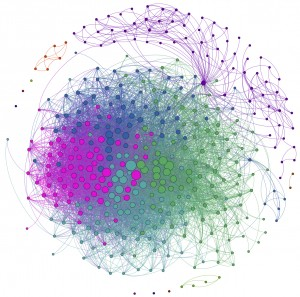
\includegraphics[width=0.5\linewidth]{../images/facebook_nonames1-300x297.jpg}
        % \caption{ Graph example.}
    \end{figure}

    \begin{note}
        {Introduce your self}
    \end{note}
\end{frame}

\begin{frame}{What do you see?}
    \begin{figure}[htp!]
        \centering
        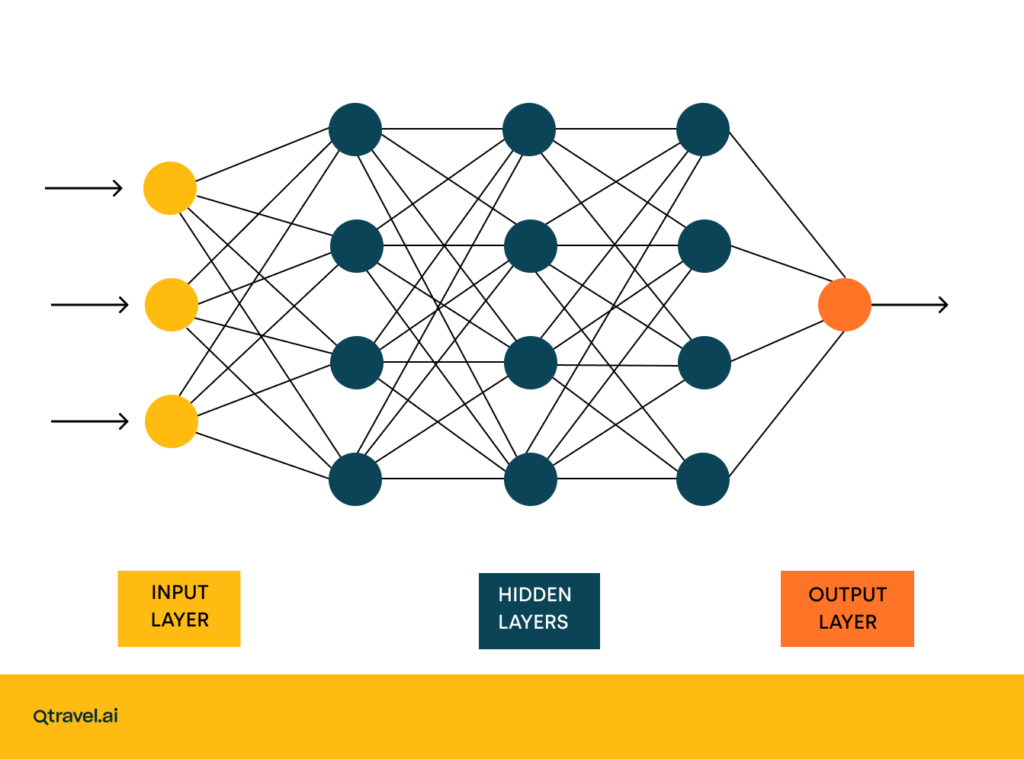
\includegraphics[
            width=0.7\linewidth,
            trim=0pt 210pt 0pt 0pt, % trim: left bottom right top.
            clip
        ]{../images/neural_networks_architecture.png}
        % \caption{Everything is connected.}
        % \vspace{-15pt}
        % \caption*{\tiny From: \url{https://www.researchgate.net/figure/Relationship-between-artificial-intelligence-machine-learning-neural-network-and-deep_fig3_354124420}} 
        % \label{fig:everything_connected}
    \end{figure}

    \begin{note}
        {Introduce your self}
    \end{note}
\end{frame}

\begin{frame}{Graph ML}
    \centering \LARGE \texttt{Graph Theory + Neural Networks}
\end{frame}

\begin{frame}
    \tableofcontents[sectionstyle=show,subsectionstyle=show/shaded/hide,subsubsectionstyle=show/shaded/hide]
    % \tableofcontents[sectionstyle=show,subsectionstyle=hide,subsubsectionstyle=hide]
\end{frame}

% Graph
\section{Graph theory}
    \begin{frame}{Motivation}
        \begin{figure}[htp!]
            \centering
            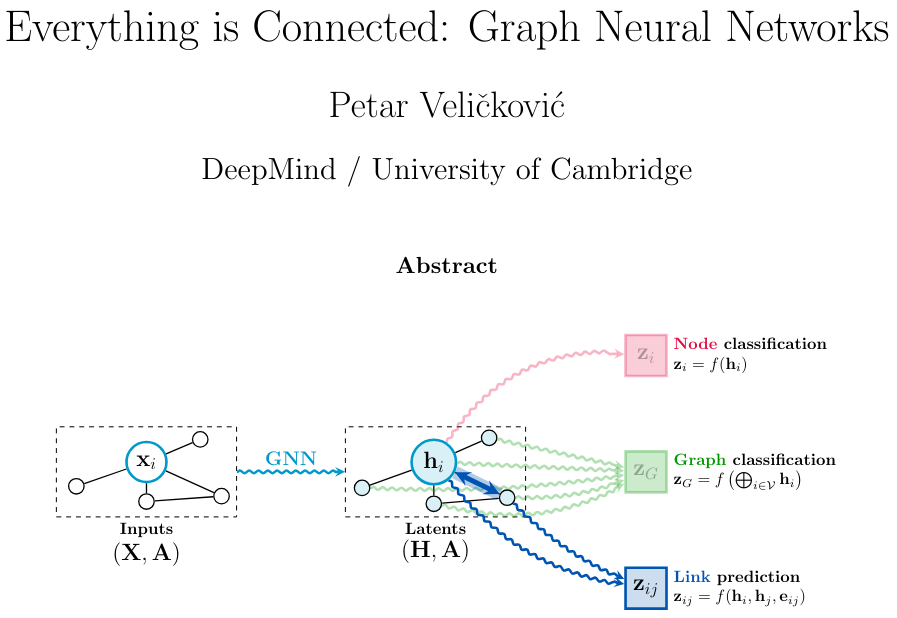
\includegraphics[
                width=0.6\linewidth,
                trim=0pt 0pt 0pt 0pt, % trim: left bottom right top.
                clip
            ]{../images/everything_is_connected.png}

            \caption{Everything is connected.}
            % \caption*{\tiny From: \url{https://www.researchgate.net/figure/Relationship-between-artificial-intelligence-machine-learning-neural-network-and-deep_fig3_354124420}} 
            \label{fig:everything_connected}
        \end{figure}

        \begin{note}
            {Introduce your self}
        \end{note}
    \end{frame}

    \begin{frame}{Graphs}
        In mathematics and computer science, a graph (network) is defined as $G = (V, E)$, where $V = \{v_1, v_2, ..., v_{n}\}$ is the nodes (or \textit{vertices}, or \textit{points}) set and $E = \{e_1, e_2, ..., e_{m}\}, e_i \in V \times V$ a set of edges (or \textit{lines}, or \textit{arcs}) formed by unordered pairs of nodes. \\

        \vspace{2mm}
        \scriptsize Number of nodes is denoted $|V|$. \\
        Number of edges is denoted $|E|$.

        \begin{figure}[ht!]
            \centering
            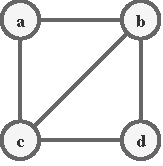
\includegraphics[width=0.2\linewidth]{../images/graph_example.pdf}
            \caption{Graph example.}
            \label{fig:graph_example}
        \end{figure}

        \begin{note}
            {Introduce your self}
        \end{note}
    \end{frame}

    \begin{frame}{Graphs}
        Furthermore, each edge $e \in E$ is said to join two vertices. If $e$ joins $u, v \in V$, then $e = (u, v)$. Vertices $u$ and $v$ are said to be adjacent. \\
        
        \begin{exampleblock}{Neighborhood}
            \begin{equation}
            \mathcal{N}(v) = \{w \in V \mid v \neq w \land (v, w) \in E\}
            \label{eq:neighborhood}
            \end{equation}
        \end{exampleblock}

        \begin{note}
            {Introduce your self}
        \end{note}
    \end{frame}

    \begin{frame}{Graphs are everywhere!}
        \begin{figure}[ht!]
            \centering
            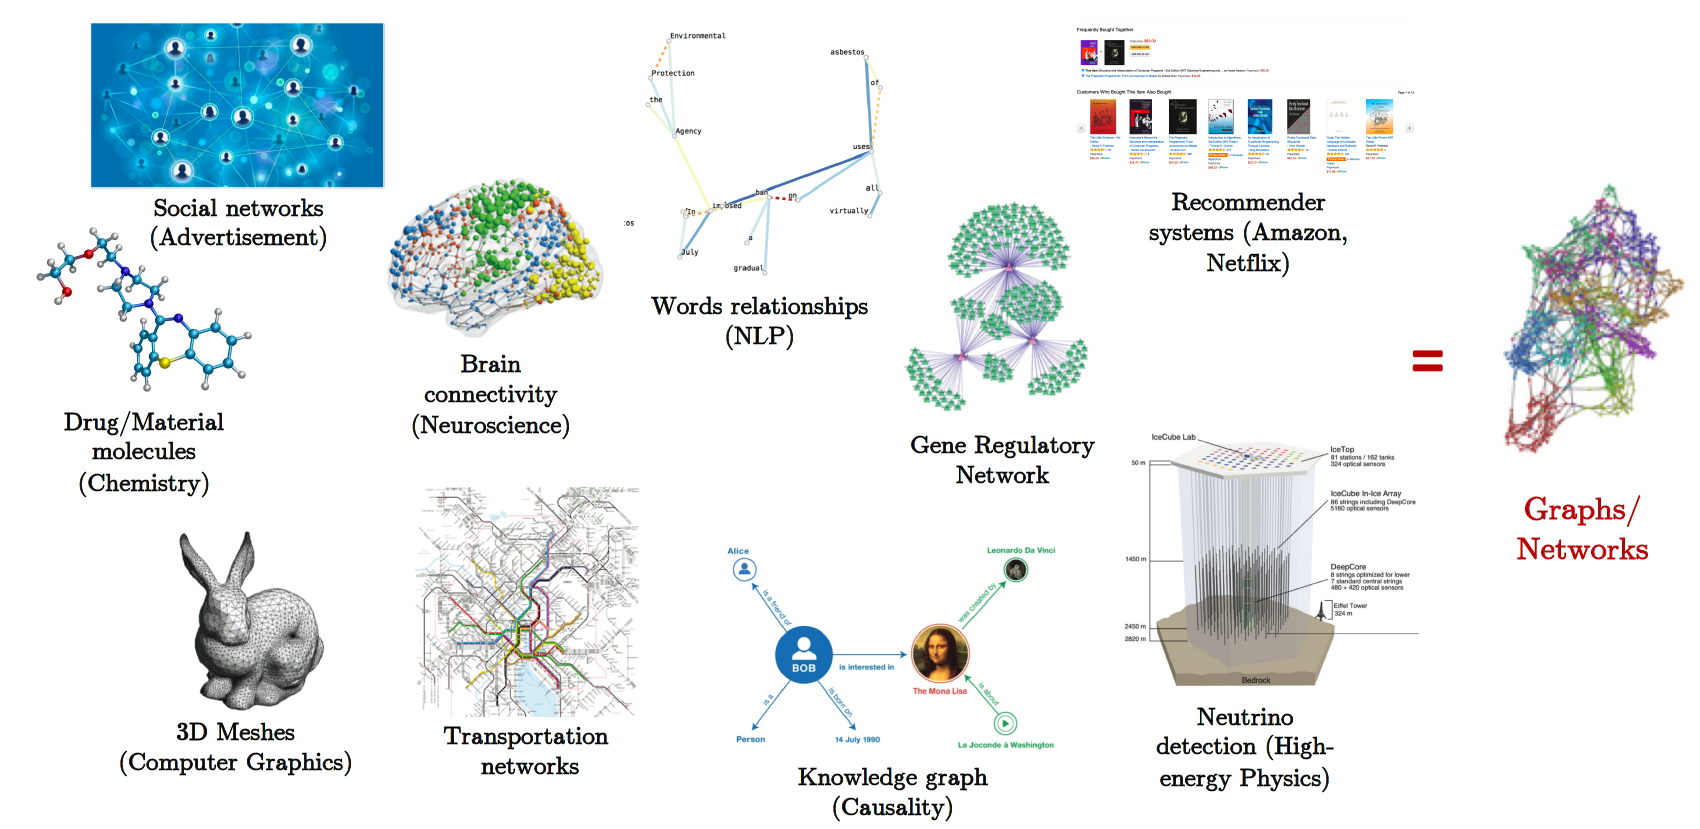
\includegraphics[width=0.9\linewidth]{../images/graph-data.png}
            \caption{\scriptsize Networks examples.}
            % From \url{https://graphdeeplearning.github.io/project/spatial-convnets/}.}
        \end{figure}
        
        \begin{note}
            {Introduce your self}
        \end{note}
    \end{frame}

    \begin{frame}{Graph representations}
        \begin{figure}
            \centering
            \begin{subfigure}{0.2\textwidth}
                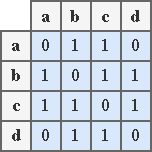
\includegraphics[width=\textwidth]{../images/graph_adjacency_matrix.pdf}
                \caption{Adjacency matrix.}
                \label{fig:graph_adjacency_matrix_}
            \end{subfigure}
            \hfill
            \begin{subfigure}{0.2\textwidth}
                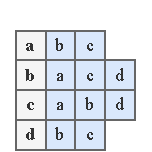
\includegraphics[width=\textwidth]{../images/graph_adjacency_list.pdf}
                \caption{Adjacency list.}
                \label{fig:graph_adjacency_list_}
            \end{subfigure}
            \hfill
            \begin{subfigure}{0.2\textwidth}
                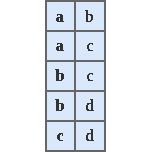
\includegraphics[width=\textwidth]{../images/graph_list_edge.pdf}
                \caption{Edge list.}
                \label{fig:graph_list_edge_}
            \end{subfigure}
            \hfill
            \begin{subfigure}{0.24\textwidth}
                
\includegraphics[width=\textwidth]{../images/incidence_matrix.pdf}
                \caption{Incidence matrix.}
                \label{fig:graph_incidence_matrix_}
            \end{subfigure}
            \hfill
            \begin{subfigure}{0.18\textwidth}
                
\includegraphics[width=\textwidth]{../images/graph_inc.pdf}
                \caption{Input graph.}
                \label{fig:graph_example_}
            \end{subfigure}
            \caption{Graph representations.}
            \label{fig:graph_representation_}
        \end{figure}

        \begin{note}
            {Write your notes here}
        \end{note}
    \end{frame}

    \begin{frame}{Types of graphs}
        \begin{columns}[t] % The "c" centered vertical alignment, "t" top vertical alignment
            \begin{column}{0.35\textwidth}
                \begin{itemize}
                    \item \alert{Based on nodes}
                    \begin{itemize}
                        \item Homogeneous
                        \item Heterogeneous
                    \end{itemize}
                \end{itemize}
            \end{column}
            
            \begin{column}{0.34\textwidth}
                \begin{itemize}
                    \item \alert{Based on edges}
                    \begin{itemize}
                        \item Undirected
                        \item Directed
                        \item Unweighted
                        \item Weighted
                        \item Sparse
                        \item Dense
                    \end{itemize}
                \end{itemize}
            \end{column}

            \begin{column}{0.32\textwidth}
                \begin{itemize}
                    \item \alert{Special types}
                    \begin{itemize}
                        \item Complete
                        \item Subgraph
                        \item Hypergraph
                        \item \textit{k}-partite
                        \item Acyclic and Cyclic
                        \item Tree
                        \item Knowledge            
                        % \item Planar
                    \end{itemize}
                \end{itemize}
            \end{column}
        \end{columns}

        \begin{note}
            {Introduce your self}
        \end{note}
    \end{frame}

    \begin{frame}{Types of graphs}
        \begin{figure}
            \centering
            \begin{subfigure}{0.241\textwidth}
                
\includegraphics[width=\textwidth]{../images/homogeneous_graph.pdf}
                \caption{Homogeneous.}
                %%% \label{fig:homogeneous_graph}
            \end{subfigure}
            \hfill
            \begin{subfigure}{0.241\textwidth}
                
\includegraphics[width=\textwidth]{../images/heterogeneous_graph.pdf}
                \caption{Heterogeneous.}
                %%% \label{fig:heterogeneous_graph}
            \end{subfigure}
            \hfill
            \begin{subfigure}{0.241\textwidth}
                
\includegraphics[width=\textwidth]{../images/directed_graph.pdf}
                \caption{Directed.}
                %%% \label{fig:directed_graph}
            \end{subfigure}
            \hfill
            \begin{subfigure}{0.241\textwidth}
                
\includegraphics[width=\textwidth]{../images/weighted_undirected_graph.pdf}
                \caption{Weighted.}
                %%% \label{fig:weighted_undirected_graph}
            \end{subfigure}
            \hfill
            \begin{subfigure}{0.16\textwidth}
                
\includegraphics[width=\textwidth]{../images/complete_graph.pdf}
                \caption{Complete.}
                %%% \label{fig:complete_graph}
            \end{subfigure}
            \hfill
            \begin{subfigure}{0.195\textwidth}
                
\includegraphics[width=\textwidth]{../images/tree.pdf}
                \caption{Tree.}
                %%% \label{fig:tree}
            \end{subfigure}
            \hfill
            \begin{subfigure}{0.11\textwidth}
                
\includegraphics[width=\textwidth]{../images/2_partite_graph.pdf}
                \caption{Bipartite.}
                %%% \label{fig:2_partite_graph}
            \end{subfigure}
            \hfill
            \begin{subfigure}{0.25\textwidth}
                
\includegraphics[width=\textwidth]{../images/knowledge_graph.pdf}
                \caption{Knowledge.}
                %%% \label{fig:knowledge_graph}
            \end{subfigure}
            \caption{Types of graphs.}
            %%% \label{fig:types_graphs}
        \end{figure}                     
    \end{frame}
    
    \begin{frame}{What type of graph is this?}
        \begin{figure}
            \centering
            \begin{subfigure}{0.26\textwidth}
                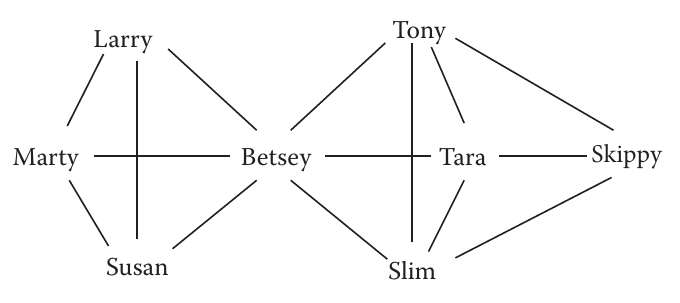
\includegraphics[width=\textwidth]{../images/social_networks.png}
                \caption{Social networks.}
                %\label{fig:social_networks}
            \end{subfigure}
            % \hfill
            \begin{subfigure}{0.27\textwidth}
                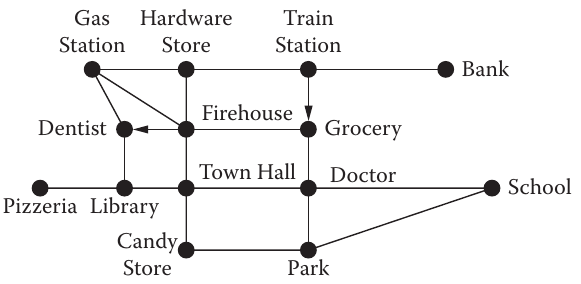
\includegraphics[width=\textwidth]{../images/road_map_landmarks.png}
                \caption{Road-map networks.}
                % \label{fig:road_map_landmarks}
            \end{subfigure}
            % \hfill
            \begin{subfigure}{0.22\textwidth}
                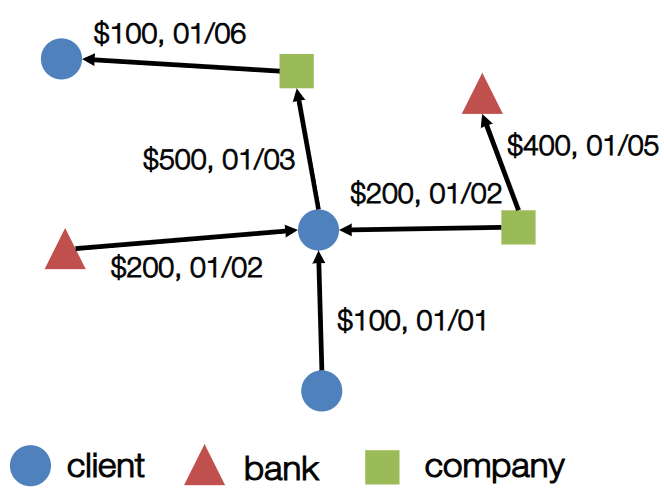
\includegraphics[width=\textwidth]{../images/financial_networks.png}
                \caption{Financial networks.}
                % \label{fig:financial_networks}
            \end{subfigure}
            % hfill
            \begin{subfigure}{0.19\textwidth}
                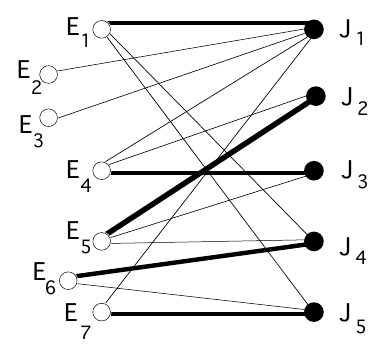
\includegraphics[width=\textwidth]{../images/personnel_assignment.png}
                \caption{Employee–job networks.}
                % \label{fig:personnel_assignment}
            \end{subfigure}
            \caption{Networks are everywhere.}
            %\label{fig:graph_everywhere}
        \end{figure}                     
    \end{frame}

    \begin{frame}{Algorithms on graphs}
        \begin{columns}[t] % The "c" centered vertical alignment, "t" top vertical alignment
            \begin{column}{0.45\textwidth}
                \begin{itemize}
                    \item \alert{Network traversal}
                    \begin{itemize}
                        \item Breadth-First Search
                        \item Depth-First Search
                    \end{itemize}
                \end{itemize}
            \end{column}
            
            \begin{column}{0.55\textwidth}
                \begin{itemize}
                    \item \alert{Shortest path algorithms}
                    \begin{itemize}
                        \item Dijkstra
                        \item Floyd–Warshall
                        \item Bellman-Ford
                    \end{itemize}
                \end{itemize}
            \end{column}
        \end{columns}

        \begin{note}
            {Introduce your self}
        \end{note}
    \end{frame}

    \begin{frame}{Breadth-First Search (BFS) algorithm}        
        \begin{columns}[t] % The "c" option specifies centered vertical alignment while the "t" option is used for top vertical alignment
            \begin{column}{0.6\textwidth}
                \begin{enumerate}
                    \item Visit the adjacent unvisited node. Mark as visited, display, and insert (queue) in a queue.
                    \item In case no adjacent node is found, remove the first node from the queue.
                    \item Repeat steps 1, and 2 until the queue is empty.
                \end{enumerate}
            \end{column}
            
            \begin{column}{0.4\textwidth}
                \begin{figure}[ht!]
                    \centering
                    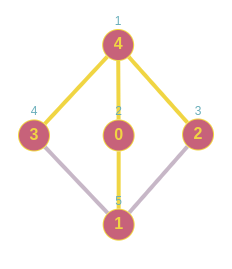
\includegraphics[width=0.7\linewidth]{../images/bfs_v1.png}
                    \caption{BFS traversal from node 4 are 4, 0, 2, 3, 1.}
                    % \caption*{Adapted from \cite{labonne2023hands}.}
                    \label{fig:bfs}
                \end{figure}
            \end{column}
        \end{columns}
        
        \begin{note}
            {Introduce your self}
        \end{note}
    \end{frame}

    \begin{frame}{Depth-First Search (DFS) algorithm}
        \begin{columns}[t] % The "c" option specifies centered vertical alignment while the "t" option is used for top vertical alignment
            \begin{column}{0.6\textwidth}
                \begin{enumerate}
                    \item Visit the adjacent unvisited node. Mark as visited, show, and push in a stack.
                    \item In case no adjacent nodes are found, all nodes in the stack that do not have adjacent nodes are popped.
                    \item Repeat steps 1, and 2 until the stack is empty.
                \end{enumerate}
            \end{column}
            
            \begin{column}{0.4\textwidth}
                \begin{figure}[ht!]
                    \centering
                    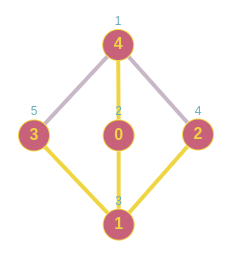
\includegraphics[width=0.7\linewidth]{../images/dfs_v1.png}
                    \caption{DFS traversal from node 4 are 4, 0, 1, 2, 3.}
                    % \caption*{Adapted from \cite{labonne2023hands}.}
                    \label{fig:dfs}
                \end{figure}
            \end{column}
        \end{columns}
        
        \begin{note}
            {Introduce your self}
        \end{note}
    \end{frame}

    \begin{frame}{Example}
        \begin{columns}[t] % Option "c" centers vertically, while "t" aligns to the top.
            \begin{column}{0.5\textwidth}
                Given the graph $G = (V, E)$, compute the BFS and DFS traversals: % the following node embedding matrix $Z \in \mathbb{R}^{5 \times 3}$:

                \begin{figure}[ht!]
                    \centering
                    
\includegraphics[width=0.4\linewidth]{../images/union.pdf}
                    \caption{Input graph.}
                    % \caption*{Adapted from \cite{labonne2023hands}.}
                    \label{fig:union}
                \end{figure}
            \end{column}
            \begin{column}{0.5\textwidth}

            \end{column}
        \end{columns}

        \begin{note}
            {Introduce your self}
        \end{note}
    \end{frame}

    \begin{frame}{Dijkstra's Algorithm}
        Dijkstra's algorithm finds the shortest path from a source node to all other nodes in a directed or undirected graph with non-negative edge weights. \newline

        \begin{exampleblock}{Idea}
            Does the shortest path from $a$ to $c$ go through $b$?
            
            \begin{figure}[ht!]
                \centering
                
\includegraphics[width=0.25\linewidth]{../images/dijkstra_idea.pdf}
                \caption{Shortest path example.}
                %%% \label{fig:dijkstra_idea}
            \end{figure}
        \end{exampleblock}
        
        % Description:
        % \begin{itemize}
        %    \item Uses a priority queue to select the closest unvisited node.
        %    \item Maintains the minimum known distance to each node.
        %    \item It is a weighted generalization of BFS.
        % \end{itemize}

        \begin{note}
            {Introduce your self}
        \end{note}
    \end{frame}

    \begin{frame}{GPS navigation and maps application}
        \begin{figure}[htp!]
            \centering
            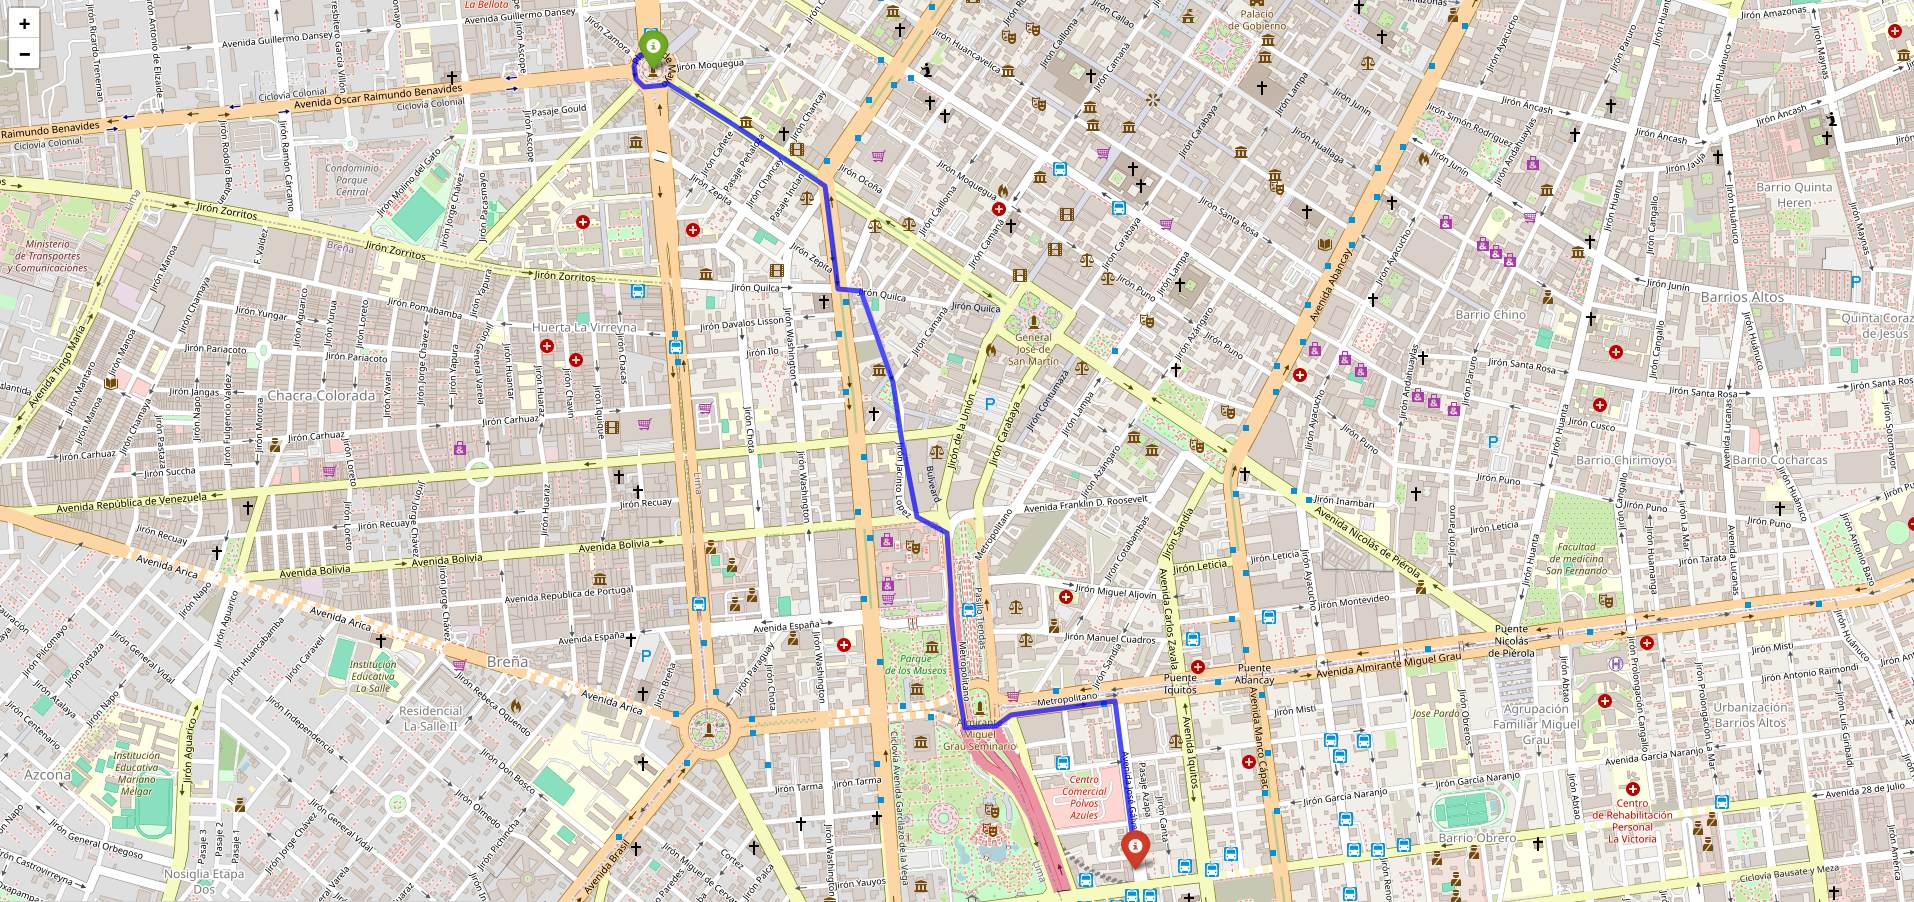
\includegraphics[width=0.9\linewidth]{../images/example_dijktra.png}
            \caption{Shortest path between two locations.}
            \label{fig:example_dijktra}
        \end{figure}

        \begin{note}
            {Introduce your self}
        \end{note}
    \end{frame}
    
    \begin{frame}{Metrics on graphs}
        \begin{columns}[t] % Option "c" centers vertically, while "t" aligns to the top.
            \begin{column}{0.33\textwidth}
                \begin{itemize}
                    \item \alert{Node-level}
                    \begin{itemize}
                        \item Degree
                        \item Degree distribution
                        \item Degree centrality
                        \item Closeness centrality
                        \item Betweenness centrality
                        % \item Centrality
                        \item Eccentricity
                        \item LCC
                    \end{itemize}
                \end{itemize}
            \end{column}
            \begin{column}{0.33\textwidth}
                \begin{itemize}
                    \item \alert{Edge-level}
                    \begin{itemize}
                        \item Shortest path
                        \item Betweenness centrality
                        \item Jaccard coefficient
                        % \item Distance
                    \end{itemize}
                \end{itemize}
            \end{column}
            \begin{column}{0.33\textwidth}
                \begin{itemize}
                    \item \alert{Graph-level}
                    \begin{itemize}
                        \item Order
                        \item Size
                        \item Density
                        \item Diameter
                        \item Radius
                        \item Average degree
                        \item Average LCC
                        \item GCC
                        \item Modularity
                    \end{itemize}
                \end{itemize}
            \end{column}
        \end{columns}

        \begin{note}
            {Introduce your self}
        \end{note}
    \end{frame}

    \begin{frame}{Node-level}
        \begin{exampleblock}{Degree}
            Given a graph $G = (V, E)$.
            
            % Number of edges incident to a node. \\

            The degree of a node $u$, denoted as $deg(u)$, is defined as the number of edges that are adjacent to this node $u$.
        \end{exampleblock}

        \begin{multicols}{2} % Two columns
            Undirected graphs:
            \begin{equation}
                deg(u) = |\{v \in V : (u, v) \in E\}|
                % \label{eq:my_equation}
            \end{equation}
        
            Directed graphs:
            \begin{equation}
                deg(u) = deg^{in}(u) + deg^{out}(u)
                % \label{eq:my_equation}
            \end{equation}
        \end{multicols}
        
        Where, $deg^{in}(u)$: in-degree and $deg^{out}(u)$: out-degree. \newline

        % Applications:
        % \begin{itemize}
        %     \item Social networks: users with many connections.
        %     \item Biology networks: metabolites involved in many reactions.
        %     \item Web: most linked pages.
        % \end{itemize}

        \begin{note}
            {Introduce your self}
        \end{note}
    \end{frame}

    \begin{frame}{Node-level}
        \begin{exampleblock}{Degree distribution}
            Given a graph $G = (V, E)$.
            
            The degree distribution of a graph $G$ is the ratio of the number of nodes with degree $k$ to the total number of nodes.
        \end{exampleblock}

        \begin{equation}
            P(k) = \frac{|V|_{k}}{|V|}
            % \label{eq:my_equation}
        \end{equation}
        
        % Applications:
        % \begin{itemize}
        %     \item Social networks: detect hubs or influencers.
        %     \item Biological networks:  identify essential genes or proteins.
        %     \item Epidemiology: predict how diseases spread over networks.
        % \end{itemize}

        \begin{note}
            {Introduce your self}
        \end{note}
    \end{frame}

    \begin{frame}{Node-level}
        \begin{exampleblock}{Betweenness centrality}
            Given a graph $G = (V, E)$.
            
            Betweenness centrality counts the number of times a particular node occurs on the shortest paths between other nodes.
            % While degree and closeness centralities are based on the concept of the person’s reachability, betweenness centrality, on the other hand, relies on the idea that a person is more important if he/she is more intermediary in the network.
        \end{exampleblock}

        \begin{equation}
            % BC(v) = {\sum_{s, t \in V,\, s \neq v \neq  t} \frac{\sigma(s, t | v)}{\sigma(s, t)}}
            BC(v) = \sum_{\substack{s,\, t \in V \\ s \neq v \neq t}} \frac{\sigma(s, t \mid v)}{\sigma(s, t)}
            % \label{eq:my_equation}
        \end{equation}

        Where $\sigma(s, t)$ is the total number of shortest paths between nodes $s$ and $t$, and $\sigma(s, t \mid v)$ is the total number of shortest paths between nodes $s$ and $t$ that passing through $v$. \newline
        
        % Applications:
        % \begin{itemize}
        %     \item Identifying bottlenecks or bridges in networks.
        %     \item Network security: Identify critical nodes for communication.
        % \end{itemize}

        \begin{note}
            {Introduce your self}
        \end{note}
    \end{frame}

    \begin{frame}{Example}
        \begin{columns}[t] % Option "c" centers vertically, while "t" aligns to the top.
            \begin{column}{0.5\textwidth}
                Given the graph $G = (V, E)$, compute the node-level metrics: % the following node embedding matrix $Z \in \mathbb{R}^{5 \times 3}$:

                \begin{figure}[ht!]
                    \centering
                    
\includegraphics[width=0.4\linewidth]{../images/union.pdf}
                    \caption{Input graph.}
                    % \caption*{Adapted from \cite{labonne2023hands}.}
                    \label{fig:union}
                \end{figure}
            \end{column}
            \begin{column}{0.5\textwidth}

            \end{column}
        \end{columns}

        \begin{note}
            {Introduce your self}
        \end{note}
    \end{frame}

    \begin{frame}{Edge-level}
        \begin{exampleblock}{Shortest path}
            Given a graph $G = (V, E)$.
            
            Shortest path between two nodes in a graph is the path with the minimum total weight.
        \end{exampleblock}
        
        Algorithms:
        \begin{itemize}
            \item Dijkstra's algorithm: for graphs with non-negative weights.
            \item Bellman-Ford: handles negative weights.
            \item Floyd-Warshall: all-pairs shortest paths.
        \end{itemize}

        % Applications:
        % \begin{itemize}
        %     \item GPS/Navigation systems: find the fastest or shortest route.
        %     \item Internet routing: determine optimal data transmission paths.
        %     \item Social networks: degrees of separation between people.
        %     \item Biology: identify efficient biochemical or signaling pathways.
        % \end{itemize}

        \begin{note}
            {Introduce your self}
        \end{note}
    \end{frame}

    \begin{frame}{Edge-level}
        \begin{exampleblock}{Betweenness centrality}
            Given a graph $G = (V, E)$.
            
            Betweenness centrality of an edge $e$ is the ratio of the shortest paths that run through $e$ to the total number of shortest paths in $G$.
        \end{exampleblock}

        \begin{equation}
            BC(e) = {\sum_{s, t \in V ,\, s \neq t} \frac{\sigma(s, t \mid e)}{\sigma(s, t)}}
            % \label{eq:my_equation}
        \end{equation}

        Here, $\sigma(s, t)$ is the total number of shortest paths between nodes $s$ and $t$, and $\sigma(s, t \mid e)$ is the number of those paths passing through $e$. \newline
        
        % Applications:
        % \begin{itemize}
        %     \item Network robustness: identify critical connections.
        %     \item Community detection: find bridges between clusters.
        %     % \item Traffic networks: detect congestion points.
        %     \item Social networks: find communication bottlenecks.
        % \end{itemize}

        \begin{note}
            {Introduce your self}
        \end{note}
    \end{frame}

    \begin{frame}{Graph-level}
        \begin{exampleblock}{Order}
            Given a graph $G = (V, E)$.
            
            The order of a graph $G$, denoted by $|V|$, is defined as the number of nodes in the graph $G$.
        \end{exampleblock}

        \begin{exampleblock}{Size}
            Given a graph $G = (V, E)$.
            
            The size of a graph $G$, denoted by $|E|$, is defined as the number of edges in the graph $G$.
        \end{exampleblock}

        \begin{note}
            {Introduce your self}
        \end{note}
    \end{frame}

    \begin{frame}{Graph-level}
        \begin{exampleblock}{Density}
            Given a graph $G = (V, E)$.
            
            Density is defined as the number of network edges divided by the maximum possible number of edges between nodes in that network. All density values are between $0$ and $1$.
        \end{exampleblock}

        \begin{equation}
            D(G) = \frac{2|E|}{|V|(|V| - 1)}
            % \label{eq:my_equation}
        \end{equation}

        % Applications:
        % \begin{itemize}
        %     \item Comparing different networks.
        %     \item Analyzing how sparse or dense a system is.
        % \end{itemize}

        \begin{note}
            {Introduce your self}
        \end{note}
    \end{frame}

    \begin{frame}{Example}
        \begin{columns}[t] % Option "c" centers vertically, while "t" aligns to the top.
            \begin{column}{0.5\textwidth}
                Given the graph $G = (V, E)$, compute the graph-level metrics: % the following node embedding matrix $Z \in \mathbb{R}^{5 \times 3}$:

                \begin{figure}[ht!]
                    \centering
                    
\includegraphics[width=0.4\linewidth]{../images/union.pdf}
                    \caption{Input graph.}
                    % \caption*{Adapted from \cite{labonne2023hands}.}
                    \label{fig:union}
                \end{figure}
            \end{column}
            \begin{column}{0.5\textwidth}

            \end{column}
        \end{columns}
        
        \begin{note}
            {Introduce your self}
        \end{note}
    \end{frame}

    \begin{frame}{Practical example: graph manipulation}
        \begin{itemize}
            \item Install requirements
                \begin{itemize}
                    \item \texttt{Python}
                    \item \texttt{Pandas}
                    \item \texttt{Numpy}
                    \item \texttt{NetworkX}
                    \item \texttt{Matplotlib}
                \end{itemize}
            \item Topics 
                \begin{itemize}
                    \item Create graphs
                    \item Metrics on graphs
                    \item Graphs visualization
                \end{itemize}
            \item Lab
                \begin{itemize}
                    \item              
                        \href{https://drive.google.com/file/d/1141_GU2KT_-lBPlyOSLzVTgYGhq_L1tJ/view?usp=sharing}{
                            \beamergotobutton{\faGoogle\ Open in Google Colab}
                        }
                \end{itemize}
        \end{itemize}

        \begin{note}
            {Introduce your self}
        \end{note}
    \end{frame}

% GML
\section{Graph machine learning}
    \subsection{Preliminaries}
        \begin{frame}{Machine learning}
            Machine learning (ML) is a field of Artificial Intelligence (AI) that studies algorithms and mathematical models capable of \alert{learning patterns from data}.

            \begin{figure}[htp!]
                \centering
                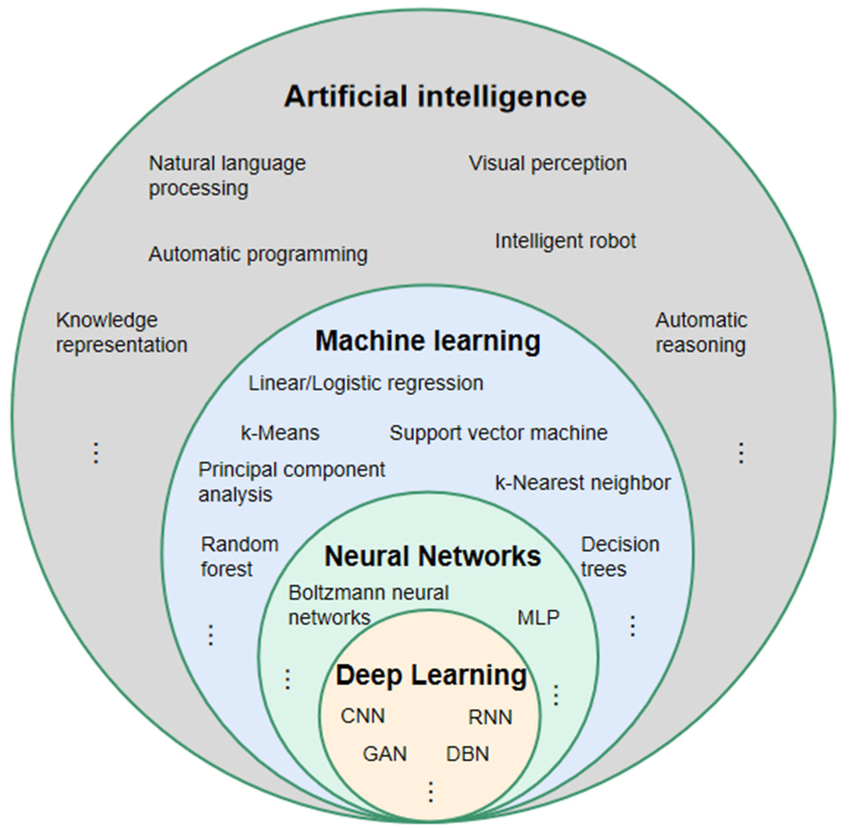
\includegraphics[
                    width=0.35\linewidth,
                    trim=0pt 0pt 0pt 0pt, % trim: left bottom right top
                    clip
                ]{../images/Relationship-between-artificial-intelligence-machine-learning-neural-network-and-deep.png}
                \caption{Relationship between AI, ML, NN, and DL.}
                \source{\url{https://www.researchgate.net/figure/Relationship-between-artificial-intelligence-machine-learning-neural-network-and-deep_fig3_354124420}}
                % \label{fig:my_image}
            \end{figure}

            \begin{note}
                {Introduce your self}
            \end{note}
        \end{frame}

        \begin{frame}{Basics of neural networks (NN)}
            \begin{figure}
                \centering
                \animategraphics[width=0.6\textwidth,loop,autoplay]
                {10} % frame rate
                {../images/NNs/8152e79cc88f4258ad55f36b09702b35uXiAdsEiqJ6Ws9wJ-} % path to figures
                {0} % start index
                {374} % end index
                \caption{Inner workings of a mathematical neuron.}
                \source{\url{https://medium.com/@jdseo/demystifying-neural-networks-an-overview-for-beginners-3688a5ded397}.}
                % \label{fig:my_image}
            \end{figure}

            \begin{note}
                {Write your notes here}
            \end{note}
        \end{frame}

        \begin{frame}{Multilayer neural networks}
            \begin{figure}[htp!]
                \centering
                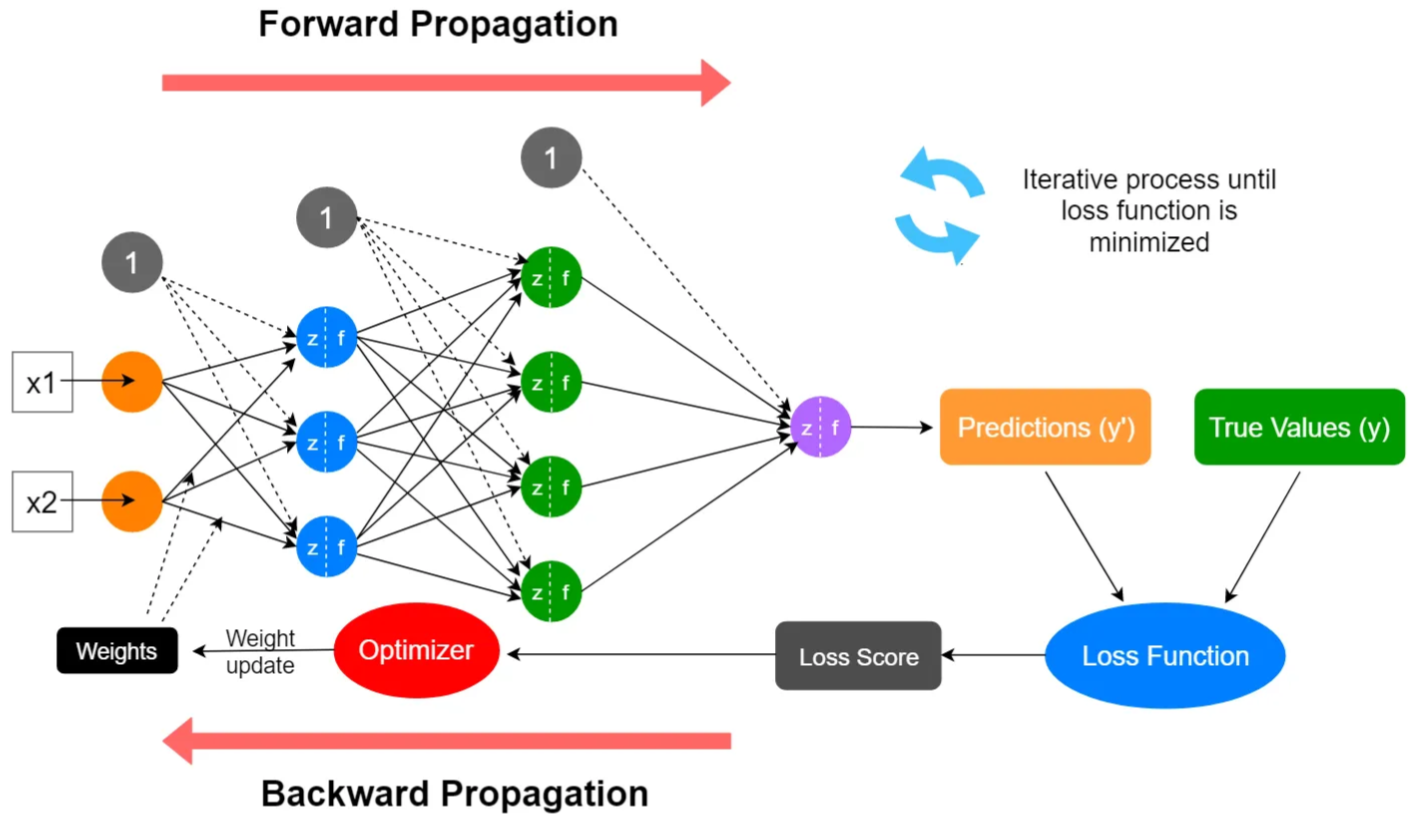
\includegraphics[
                    width=0.7\linewidth,
                    trim=0pt 0pt 0pt 0pt, % trim: left bottom right top
                    clip
                ]{../images/neural_networks.png}
                \caption{Neural networks learning.}
                \source{\url{https://medium.com/data-science-365/overview-of-a-neural-networks-learning-process-61}}
                % \label{fig:my_image}
            \end{figure}

            \begin{note}
                {Introduce your self}
            \end{note}
        \end{frame}

        \begin{frame}{Example of NN}
            \begin{figure}
                \centering
                \animategraphics[width=0.7\textwidth,loop,autoplay]
                {5} % frame rate
                {../images/network-propagation/network-propagation_} % path to figures
                {0} % start index
                {71} % end index
                \caption{Image classification.}
                \source{\url{https://www.3blue1brown.com/lessons/neural-networks}.}
                % \label{fig:my_image}
            \end{figure}

            \begin{note}
                {Write your notes here}
            \end{note}
        \end{frame}

        \begin{frame}{Representation learning}
            \begin{itemize}
                \item Word embeddings
                \begin{itemize}
                    \item Word2Vec
                    \begin{itemize}
                        \item \alertplain{Skip-Gram}
                        \item Continuous Bag of Words (CBOW)
                    \end{itemize}
                \end{itemize}
                \item Graph embeddings
                \begin{itemize}
                    \item Shallow embeddings
                    \begin{itemize}
                        \item \alertplain{DeepWalk}
                        \item \alertplain{Node2vec}
                        \item Struc2vec
                        \item Structural Deep Network Embedding (SDNE)
                        \item Metapath2vec
                    \end{itemize}
                    \item Graph Neural Networks (GNN)
                    \begin{itemize}
                        \item \alert{Graph Convolutional Networks} (GCN)
                        \item Graph Attention Networks (GAT)
                        \item Graph Isomorphism Networks (GIN)
                        \item GraphSAGE
                        \item Graph Autoencoders (GAE)
                        % \item Graph Transformers
                    \end{itemize}
                \end{itemize}
            \end{itemize}

            \begin{note}
                {Introduce your self}
            \end{note}
        \end{frame}

        \begin{frame}{Word embedding}
            \begin{figure}
                \centering
                \animategraphics[width=0.7\textwidth,loop,autoplay]
                {1} % frame rate
                {../images/word_embedding/frame-} % path to figures
                {0} % start index
                {4} % end index
                \caption{How it works.}
                \source{\url{https://lena-voita.github.io/nlp_course/word_embeddings.html}.}
                % \label{fig:my_image}
            \end{figure}

            \begin{note}
                {Write your notes here}
            \end{note}
        \end{frame}

        \begin{frame}{Word2vec} % \cite{mikolov2013efficient}}
            % https://dl.acm.org/doi/pdf/10.1145/2623330.2623732
            % https://arxiv.org/pdf/1301.3781
            \alert{Word2vec}: Efficient Estimation of Word Representations in Vector Space
            
            {\scriptsize (Mikolov, T., Chen, K., Corrado, G., \& Dean, J., 2013)}
            
            \begin{figure}[htp!]
                \centering
                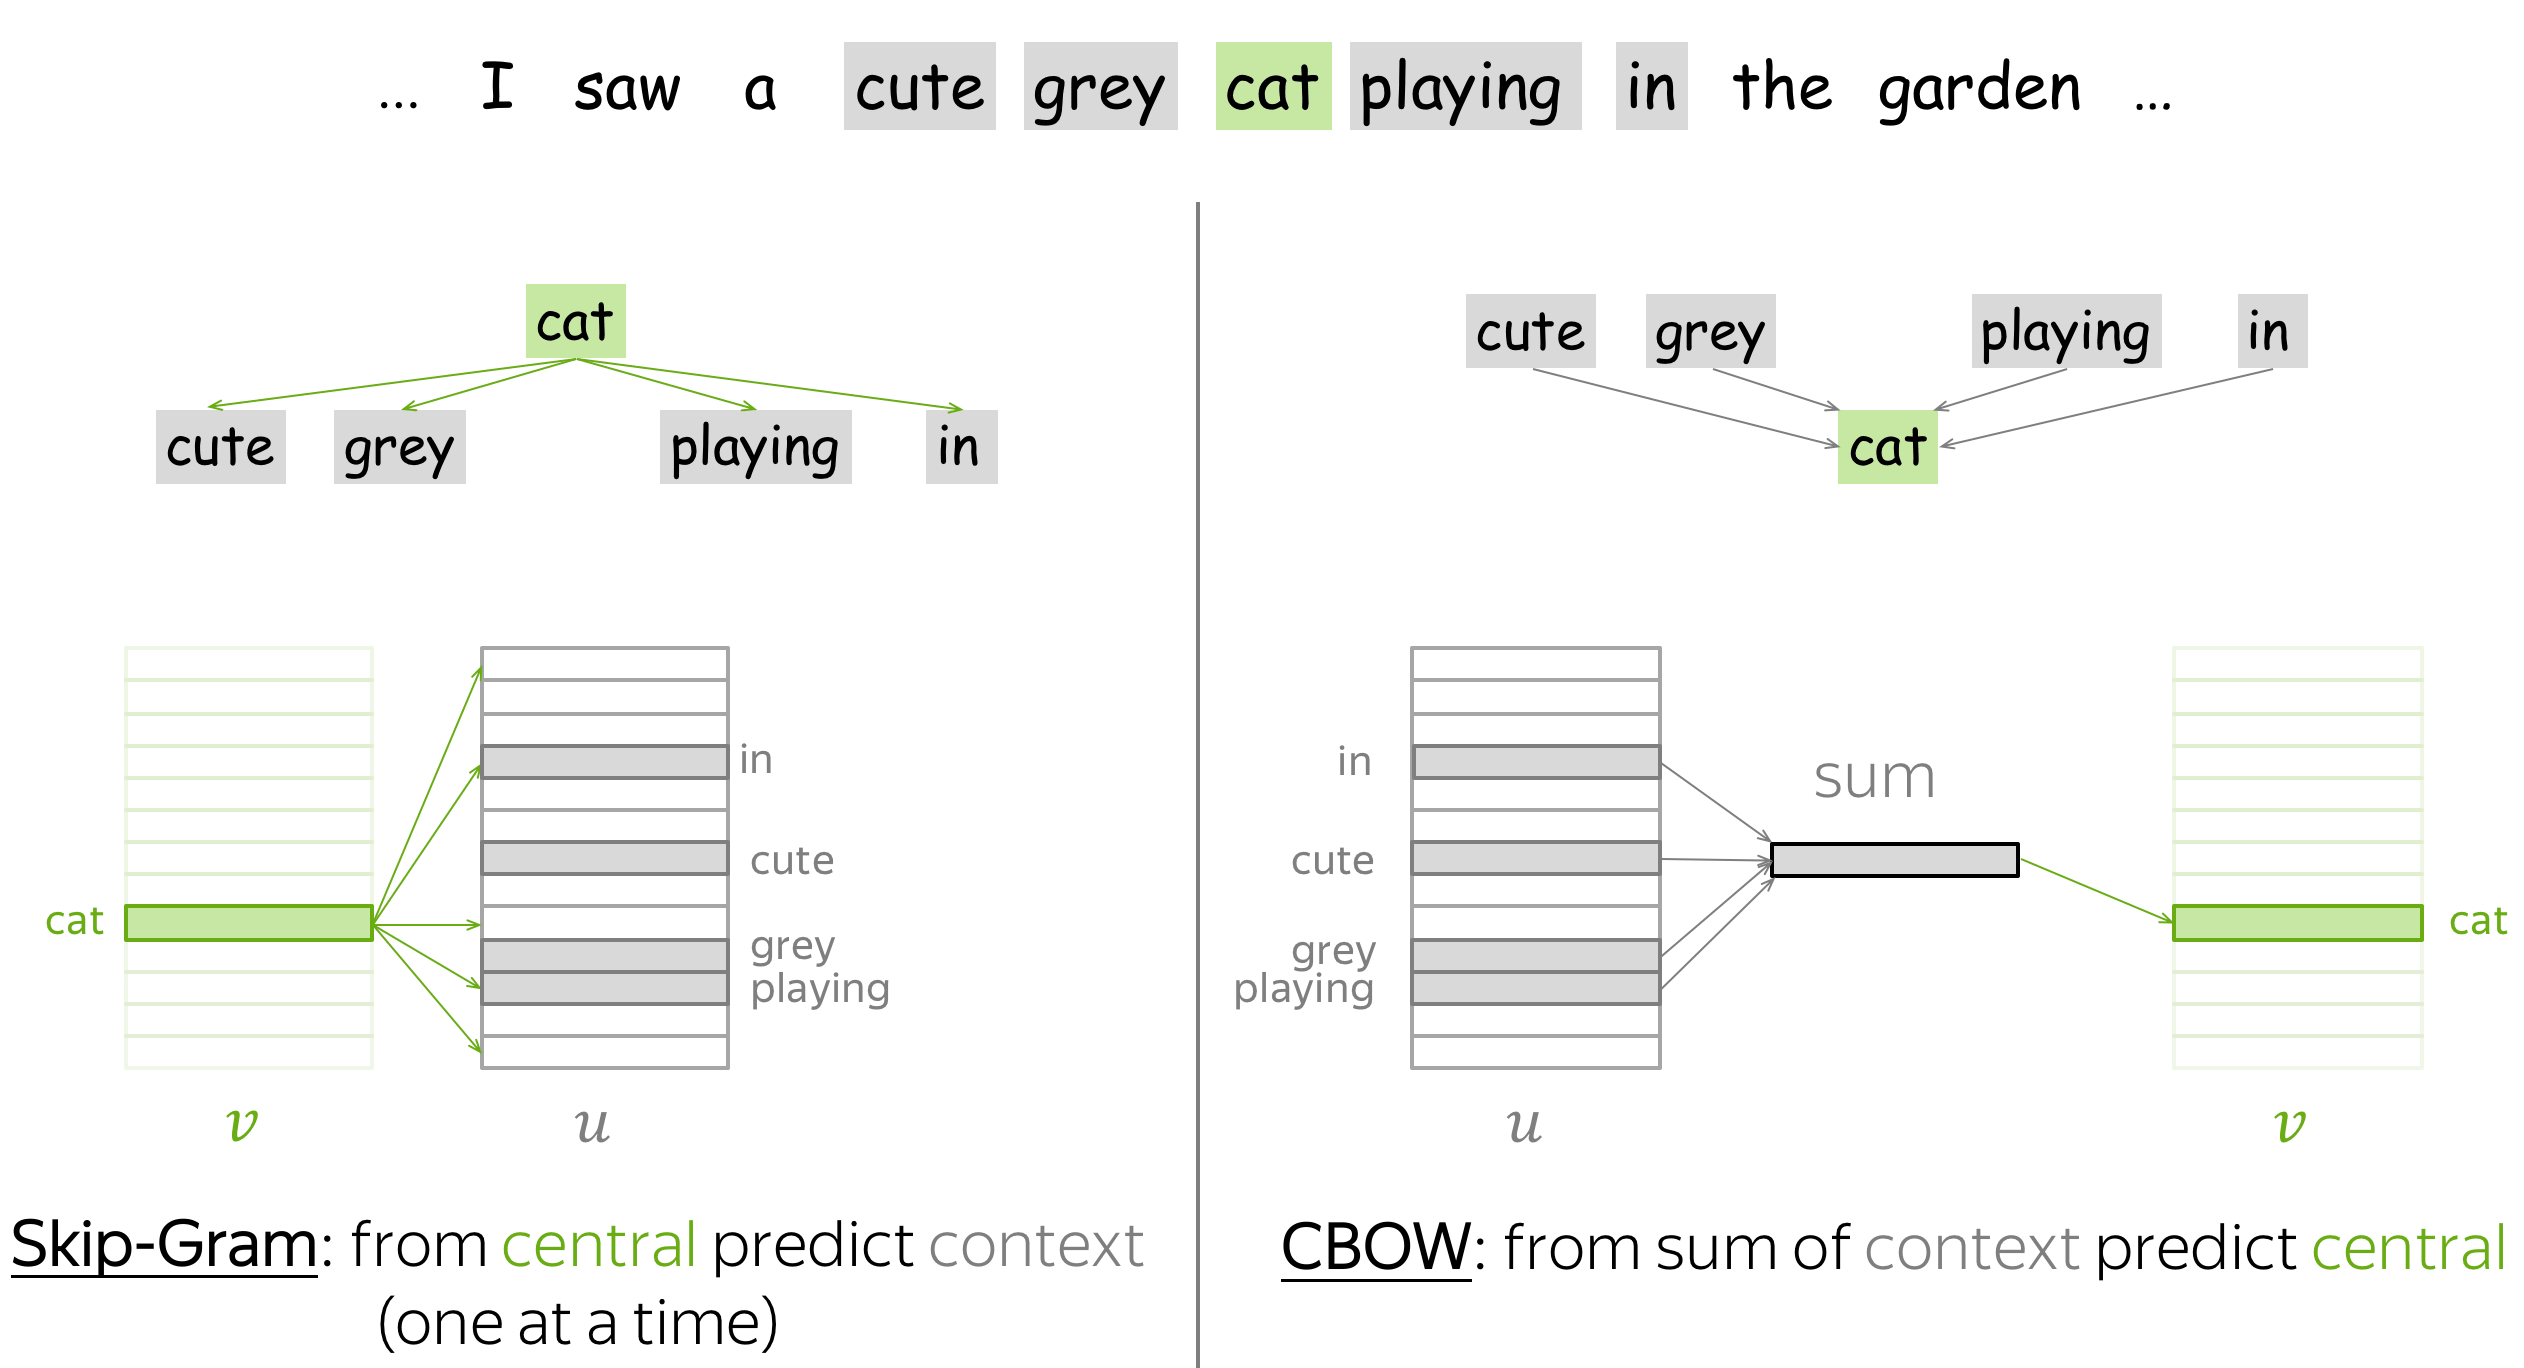
\includegraphics[
                    width=0.65\linewidth,
                    trim=0pt 0pt 0pt 0pt, % trim: left bottom right top
                    clip
                ]{../images/cbow_skip-min.png}
                \caption{Skip-gram and CBOW.}
                \source{\url{https://lena-voita.github.io/nlp_course/word_embeddings.html}}
                % \label{fig:my_image}
            \end{figure}

            \begin{note}
                {Introduce your self}
            \end{note}
        \end{frame}

        \begin{frame}{Skip-gram}
            \begin{figure}[htp!]
                \centering
                \includegraphics[
                    width=0.8\linewidth,
                    trim=0pt 0pt 0pt 0pt, % trim: left bottom right top
                    clip
                ]{../images/Word2Vec.png}
                \caption{Skip-gram architecture.}
                % \source{\url{https://medium.com/@infocean.info/the-machine-learning-pipeline-b8a9ebbc63d1}}
                % \label{fig:my_image}
            \end{figure}

            \begin{note}
                {Introduce your self}
            \end{note}
        \end{frame}

        \begin{frame}{Word2vec output}
            \begin{figure}[htp!]
                \centering
                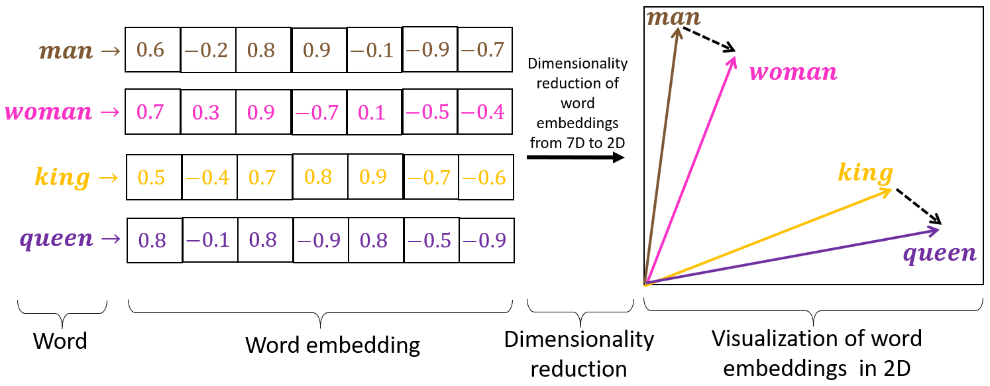
\includegraphics[
                    width=0.7\linewidth,
                    trim=0pt 0pt 0pt 0pt, % trim: left bottom right top
                    clip
                ]{../images/skip-gram_result.png}
                \caption{Word embeddings output.}
                \source{\url{https://doi.org/10.1371/journal.pone.0231189.g008}}
                % \label{fig:my_image}
            \end{figure}

            \begin{note}
                {Introduce your self}
            \end{note}
        \end{frame}

        \begin{frame}{Similarity analysis}
            \begin{alertblock}{Cosine similarity}
                \begin{equation}
                    cos(\theta) = \text{sim}(z_u, z_v) = \frac{z_u.z_v}{\|z_u\|\|z_v\|}
                    % \label{eq:my_equation}
                \end{equation}
            \end{alertblock}

            \begin{figure}[htp!]
                \centering
                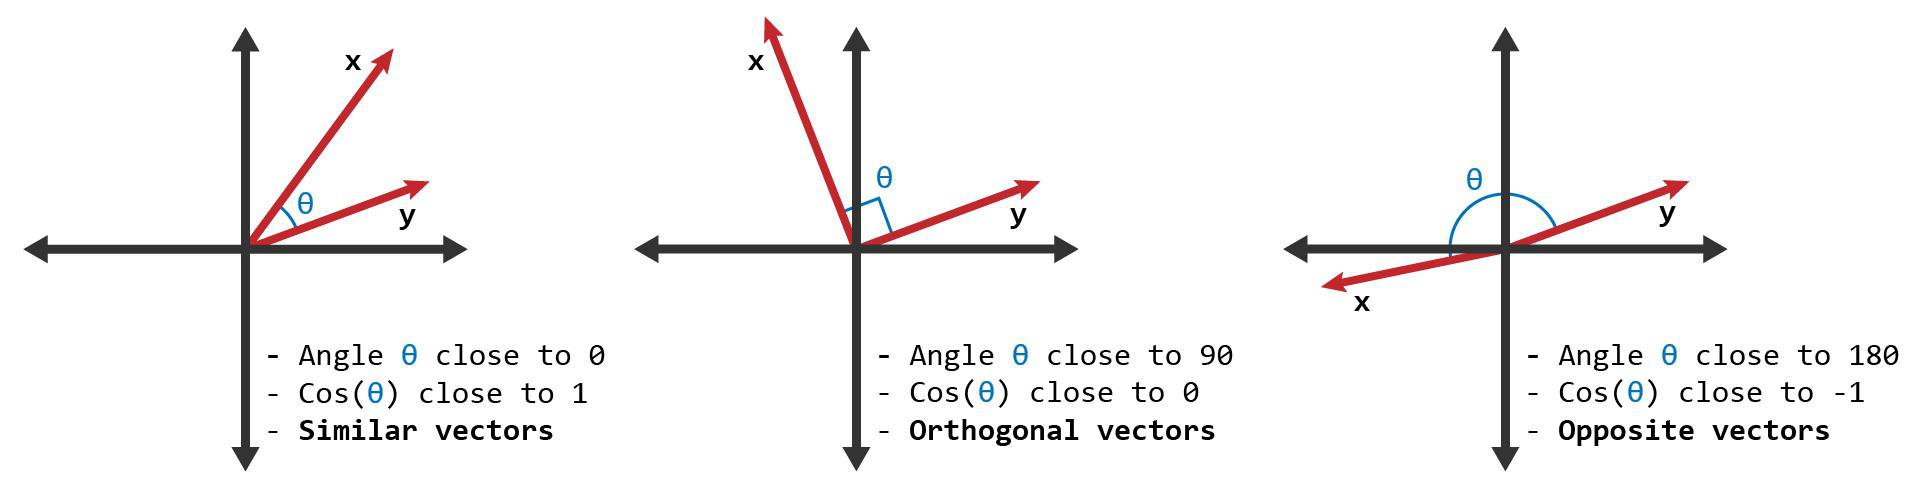
\includegraphics[
                    width=0.9\linewidth,
                    trim=0pt 0pt 0pt 0pt, % trim: left bottom right top
                    clip
                ]{../images/cosine_similarity_vectors.jpg}
                \caption{Cosine similarity interpretation.}
                \source{\url{https://www.learndatasci.com/glossary/cosine-similarity/}}
                % \label{fig:my_image}
            \end{figure}

            \begin{note}
                {Introduce your self}
            \end{note}
        \end{frame}

    \subsection{Shallow embeddings}
        \begin{frame}{Graph embeddings}
            % A \textit{node embedding} is formally defined as a function $f: V \rightarrow \mathbb{R}^{d}$ that maps each node of the graph $G = (V, E)$ to a low-dimensional vector representation, preserving relevant structural properties of the graph. \newline
            % The resulting set $Z = \{z_1, z_2, \ldots, z_{|V|}\}$, where each $z_i = f(v_i) \in \mathbb{R}^{d}$ is called a \alert{node embedding}, and the matrix $Z \in \mathbb{R}^{|V| \times d}$ is referred to as the \textit{embedding matrix}. The parameter $d$ denotes the embedding dimension, satisfying $d \ll |V|$.
            \begin{exampleblock}{Node-level embedding}
                It is a function $f: V \rightarrow \mathbb{R}^{d}$ that maps each node of the graph $G = (V, E)$ to a low-dimensional vector ($d \ll \left| V \right|$), preserving the structural properties of the graph, where $z_i = f(v_i) \in \mathbb{R}^{d}$ and $Z \in \mathbb{R}^{\left| V \right| \times d}$ are called \alertplain{node embedding} and \alertplain{embedding matrix}, respectively.
            \end{exampleblock}

            \begin{figure}[htp!]
                \centering
                
\includegraphics[
                    width=0.7\linewidth,
                    trim=0pt 0pt 0pt 0pt, % trim: left bottom right top
                    clip
                ]{../images/shallow_embeddings.pdf}
                \caption{Shallow embeddings scheme.}
                % \source{Author, 2024.}
                % \label{fig:my_image}
            \end{figure}

            \begin{note}
                {Introduce your self}
            \end{note}
        \end{frame}

        \begin{frame}{DeepWalk}
            % https://dl.acm.org/doi/pdf/10.1145/2623330.2623732
            \alert{DeepWalk}: Online Learning of Social Representations
            
            {\scriptsize (Perozzi, B., Al-Rfou, R., \& Skiena, S., 2014)}

            \begin{figure}[htp!]
                \centering
                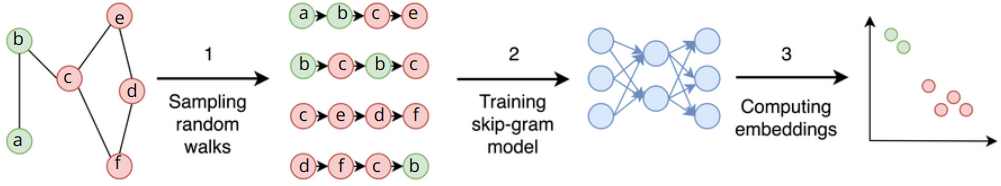
\includegraphics[
                    width=0.9\linewidth,
                    trim=0pt 0pt 0pt 0pt, % trim: left bottom right top
                    clip
                ]{../images/deepwalk.png}
                \caption{DeepWalk workflow.}
                % \source{Author, 2024.} grover2016node2vec
                % \label{fig:my_image}
            \end{figure}

            Parameters:
            \begin{itemize}
                \item walks per node: $\gamma = \underline{\hspace{1cm}}$
                \item walk length: $n = \underline{\hspace{1cm}}$
                \item embedding dimension: $d = \underline{\hspace{1cm}}$
            \end{itemize}
            % \begin{description}
            %     \item [Walks per node:] $\gamma = ?$
            %     \item [Walk length:] $t = ?$
            %     \item [Embedding dimension:] $d = ?$
            % \end{description}

            \begin{note}
                {Introduce your self}
            \end{note}
        \end{frame}

        \begin{frame}{Node2vec}
            % https://dl.acm.org/doi/pdf/10.1145/2939672.2939754
            \alert{Node2vec}: Scalable Feature Learning for Networks
            
            {\scriptsize (Grover and Leskovec, 2016)}

            \begin{figure}[htp!]
                \centering
                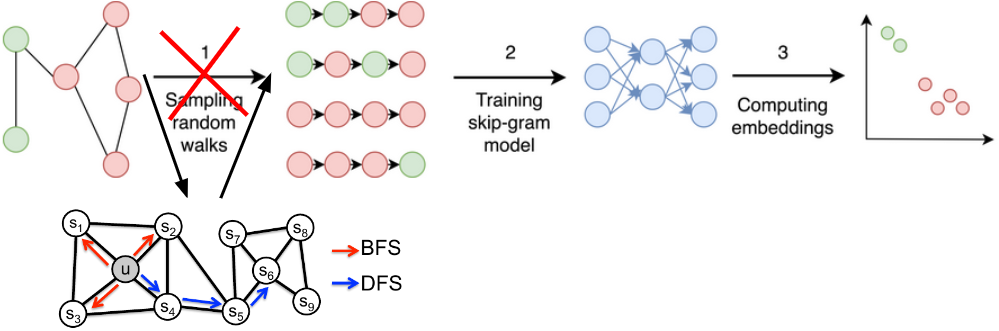
\includegraphics[
                    width=0.69\linewidth,
                    trim=0pt 0pt 0pt 0pt, % trim: left bottom right top
                    clip
                ]{../images/node2vec.png}
                \caption{Node2vec workflow.}
                % \source{Author, 2024.}
                % \label{fig:my_image}
            \end{figure}

            \begin{columns}[t] % Option "c" centers vertically, while "t" aligns to the top.
                \begin{column}{0.4\textwidth}
                    Parameters:
                    \begin{itemize}
                        \item walks per node: $\gamma = 1$
                        \item walk length: $n = 3$
                        \item embedding dimension: $d = 2$
                    \end{itemize}
                \end{column}
                
                \begin{column}{0.6\textwidth}
                    New parameters:
                    \begin{itemize}
                        \item BFS (local microscopic view): $p = 1$, $q = 2$
                        \item DFS (global macroscopic view): $p = 1$, $q = 0.5$
                    \end{itemize}
                \end{column}
            \end{columns}

            % Parameters:
            % \begin{multicols}{2} % Two columns
            %     \footnotesize
            %     \begin{itemize}
            %         \item walks per node: $\gamma = 1$
            %         \item walk length: $t = 4$
            %         \item embedding dimension: $d = 2$
            %         \item BFS (local microscopic view): $p = 1$, $q = 2$
            %         \item DFS (global macroscopic view): $p = 1$, $q = 0.5$
            %     \end{itemize}
            %     % BFS-like walk: Low value of 𝑝
            %     % DFS-like walk: Low value of 𝑞
            % \end{multicols}

            \begin{note}
                {Introduce your self}
            \end{note}
        \end{frame}
        
        \begin{frame}{Limitations of Shallow embeddings}
            Shallow embedding methods have three key limitations:

            \begin{enumerate}
                \item \alert{No parameter sharing}: each node has a unique embedding vector, making the approach statistically and computationally inefficient, with a parameter complexity of $\mathcal{O} (∣V∣)$ that becomes intractable for large graphs. % GNN, O(d2×L)
                \item \alert{No node features}: shallow methods ignore node attribute information during encoding, missing potentially valuable feature information available in many graph datasets.
                \item \alert{Transductive}: embeddings can only be generated for nodes seen during training, making these methods unable to generalize to unseen nodes in inductive settings.
            \end{enumerate}

            \begin{note}
                {Introduce your self}
            \end{note}
        \end{frame}

    \subsection{Graph neural networks (GNNs)}
        \begin{frame}{Graph Neural Networks (GNN)}
            % A \textit{node embedding} is formally defined as a function $f: V \rightarrow \mathbb{R}^{d}$ that maps each node of the graph $G = (V, E)$ to a low-dimensional vector representation, preserving relevant structural properties of the graph. \newline
            % The resulting set $Z = \{z_1, z_2, \ldots, z_{|V|}\}$, where each $z_i = f(v_i) \in \mathbb{R}^{d}$ is called a \alert{node embedding}, and the matrix $Z \in \mathbb{R}^{|V| \times d}$ is referred to as the \textit{embedding matrix}. The parameter $d$ denotes the embedding dimension, satisfying $d \ll |V|$.

            % It is a function $f: (A, X) \rightarrow H$ that maps each node $v_i \in V$ of the graph $G = (V, E)$ to a low-dimensional vector ($d \ll \left| V \right|$), preserving relevant structural properties of the graph. Here $A \in \mathbb{R}^{|V| \times |V|}$ is the adjacency matrix of $G$, $X \in \mathbb{R}^{|V| \times C}$ is the node features matrix, and $H^{(l)} = Z$ with $z_i = f(v_i) \in \mathbb{R}^{d}$ and $Z \in \mathbb{R}^{|V| \times d}$. % are called \alertplain{node embedding} and \alertplain{embedding matrix}, respectively.

            % It is a function $f: (A, X) \rightarrow H$ that maps each node $v_i \in V$ of the graph $G = (V, E)$ to a low-dimensional vector ($d \ll |V|$), preserving relevant structural properties of the graph. Here $A \in \mathbb{R}^{|V| \times |V|}$ is the adjacency matrix of $G$, and $X \in \mathbb{R}^{|V| \times C}$ is the node feature matrix, where $C$ is the number of input features per node. The output of the $l$-th layer of the neural network is denoted $H^{(l)} \in \mathbb{R}^{|V| \times d}$, where $l \in \{0, 1, \dots, L\}$ indexes the depth of the network, such that $H^{(0)} = X$ is the initial input and the final representation $Z = H^{(L)}$ is the learned embedding matrix, with each row $z_i = f(v_i) \in \mathbb{R}^{d}$ corresponding to the embedding of node $v_i$.

            % A GNN is a function $f: (A, X) \rightarrow Z$ that maps each node $v \in V$ of a graph $G = (V, E)$ to a low-dimensional embedding $\mathbf{z}_v = f(v) \in \mathbb{R}^{d}$, where $d \ll |V|$.

            % The inputs are defined as follows: $A \in \mathbb{R}^{|V| \times |V|}$ is the adjacency matrix, $X \in \mathbb{R}^{|V| \times C}$ is the node feature matrix, and $C$ denotes the feature dimensionality. The output $\mathbf{Z} = H^{(L)} \in \mathbb{R}^{|V| \times d}$ is the final node embedding matrix, where $\mathbf{z}_v = \mathbf{h}_{v}^{(L)}$ is the embedding of node $v$ at the last layer $L$. The index $l \in \{0, 1, \dots, L\}$ denotes the network layer, with $H^{(0)} = X$ as the initialization.

            \begin{exampleblock}{Node-level embedding}
                It is a function $f: (A, X) \rightarrow Z$ that maps each node $v \in V$ of a graph $G = (V, E)$ to a low-dimensional embedding $z_v \in \mathbb{R}^{d}$ ($d \ll |V|$). \\
            
                Here $A \in \mathbb{R}^{|V| \times |V|}$ is the adjacency matrix, $X \in \mathbb{R}^{|V| \times C}$ is the node feature matrix, $C$ denotes the feature dimensionality, and $Z = H^{(L)} \in \mathbb{R}^{|V| \times d}$ is the final embedding matrix obtained after $L$ layers, with $H^{(0)} = X$.
            \end{exampleblock}

            \begin{figure}[htp!]
                \centering
                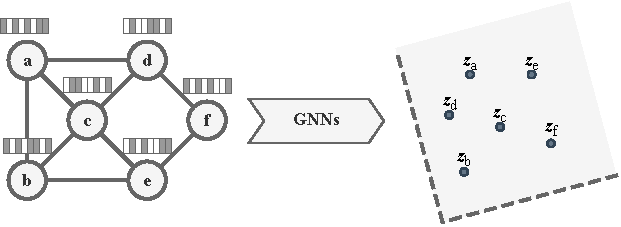
\includegraphics[
                    width=0.7\linewidth,
                    trim=0pt 0pt 0pt 0pt, % trim: left bottom right top
                    clip
                ]{../images/graph_neural_networks.pdf}
                \caption{GNNs scheme.}
                % \source{Author, 2024.}
                % \label{fig:my_image}
            \end{figure}

            \begin{note}
                {Introduce your self}
            \end{note}
        \end{frame}

        \begin{frame}{How GNNs works?}
            \begin{figure}[htp!]
                \centering
                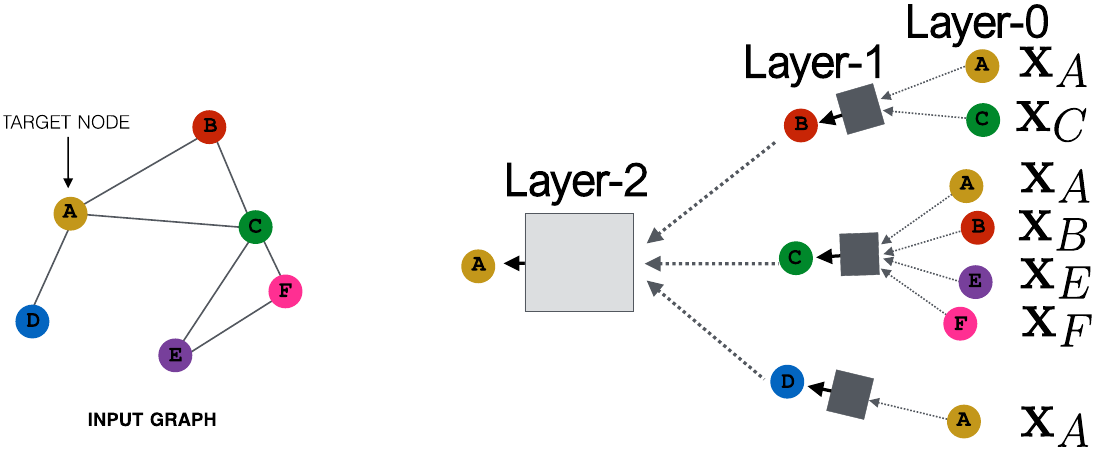
\includegraphics[
                    width=0.7\linewidth,
                    trim=0pt 0pt 0pt 0pt, % trim: left bottom right top
                    clip
                ]{../images/computacional_graph_layers.png}
                \caption{Computation graph representation and layers.}
                \source{\url{https://web.stanford.edu/class/cs224w/}.}
                % \label{fig:my_image}
            \end{figure}

            \begin{note}
                {Introduce your self}
            \end{note}
        \end{frame}

        \begin{frame}{Computacional graphs}
            \begin{figure}[htp!]
                \centering
                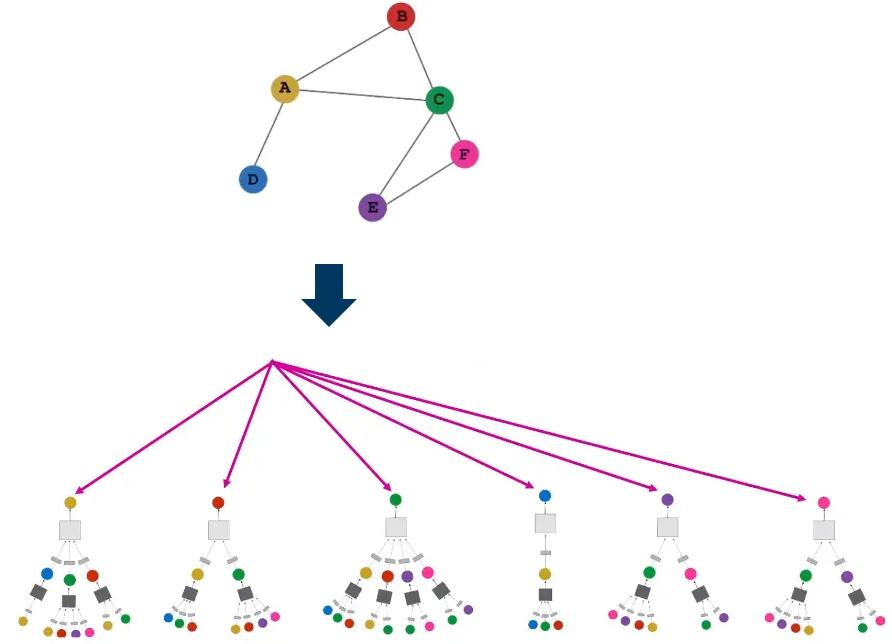
\includegraphics[
                    width=0.6\linewidth,
                    trim=0pt 0pt 0pt 0pt, % trim: left bottom right top
                    clip
                ]{../images/gnn_computacional_graphs.jpg}
                \caption{Example of computacional graph.}
                \source{\url{https://web.stanford.edu/class/cs224w/}.}
                % \label{fig:my_image}
            \end{figure}

            \begin{note}
                {Introduce your self}
            \end{note}
        \end{frame}

        \begin{frame}{Message passing mechanism}
            % https://www.tensortonic.com/ml-math/graph-theory/message-passing
            % https://distill.pub/2021/gnn-intro/
            % https://apxml.com/courses/introduction-to-graph-neural-networks/chapter-2-the-message-passing-mechanism
            % https://arxiv.org/pdf/2006.00144
            % https://apxml.com/courses/introduction-to-graph-neural-networks/chapter-2-the-message-passing-mechanism/general-gnn-layer-aggregate-update
            % https://apxml.com/courses/graph-neural-networks-gnns/chapter-1-gnn-foundations-revisited/message-passing-revisited
            % https://www.youtube.com/watch?v=cx9Dn_tGLz4
            % https://pytorch-geometric.readthedocs.io/en/latest/notes/create_gnn.html#:~:text=x%20i%20(%20k%20)%20%3D%20%CE%B3,MLPs%20(Multi%20Layer%20Perceptrons).
            % https://kumo.ai/pyg/concepts/message-passing/

            % The general message passing process consists of three steps:
            % The message passing mechanism consists of three successive operations per layer $l \in \{1, \dots, L\}$:
            The message passing mechanism consists of two steps (compressed version) per layer $l \in \{1, \dots, L\}$:

            \begin{enumerate}
                \item Message function
                \item Aggregation function
                % \item Update function
            \end{enumerate}

            \begin{figure}[htp!]
                \centering
                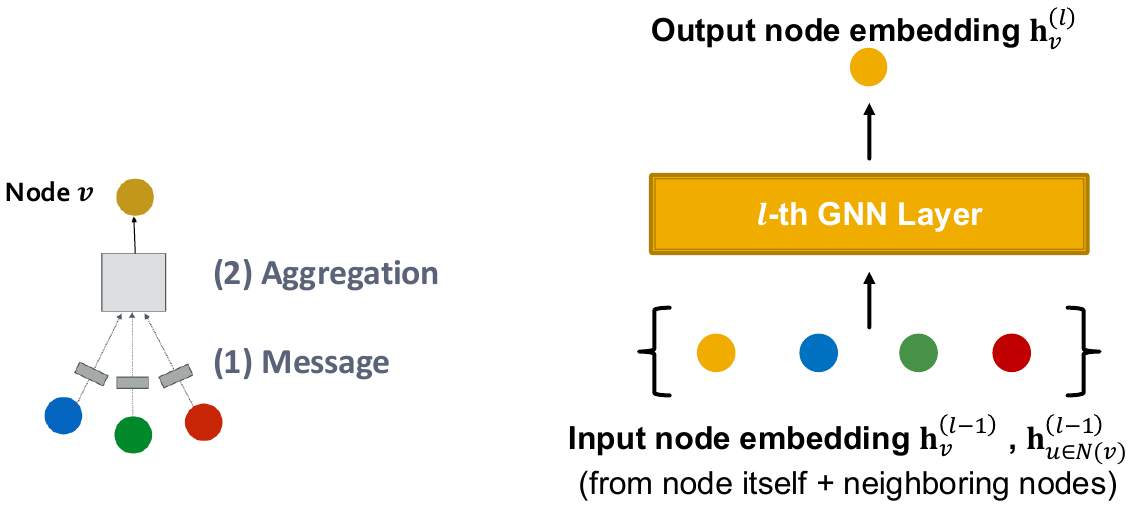
\includegraphics[
                    width=0.65\linewidth,
                    trim=0pt 0pt 0pt 0pt, % trim: left bottom right top
                    clip
                ]{../images/single_gnn_layer.png}
                \caption{Single layer of GNN.}
                \source{\url{https://web.stanford.edu/class/cs224w/}.}
                % \label{fig:my_image}
            \end{figure}

            \begin{note}
                {Introduce your self}
            \end{note}
        \end{frame}

        \begin{frame}{Message passing mechanism}
            \begin{alertblock}{Message function}
                For each node $u \in V$, a message $m_u^{(l)}$ is computed from its own representation at the previous layer $h_u^{(l-1)}$. A common example is a linear transformation:

                % For each node $u \in V$, a message $m_u^{(l)}$ is computed from the representations of its neighboring nodes $v \in \mathcal{N}(u)$ at the previous layer $h_v^{(l-1)}$. A common example is a linear transformation:

                \begin{equation}
                    % m_{u}^{(l)} = \text{MESSAGE}^{(l)}\left(h_u^{(l-1)}\right) = W^{(l)}\, h_u^{(l-1)}
                    m_{u}^{(l)} = \text{MESSAGE}^{(l)}\left(h_u^{(l-1)}\right) = h_u^{(l-1)}W^{(l)}
                    % \label{eq:equation1}
                \end{equation}

                % where $W^{(l)} \in \mathbb{R}^{d \times d}$ is a learnable weight matrix.
            \end{alertblock}

            \begin{figure}[htp!]
                \centering
                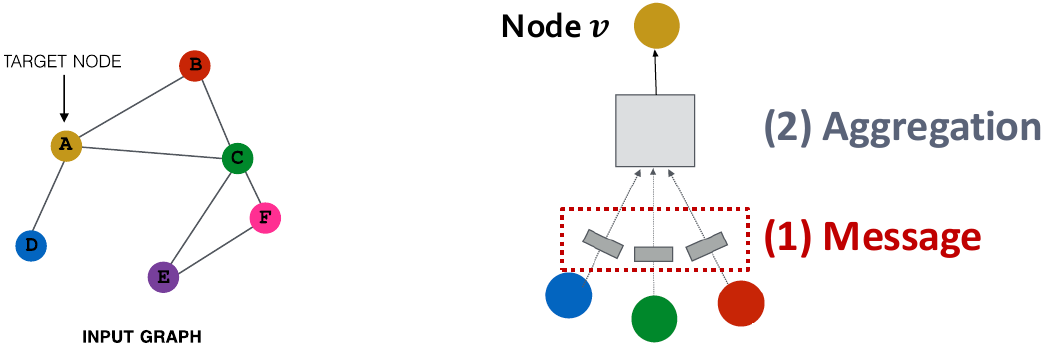
\includegraphics[
                    width=0.55\linewidth,
                    trim=0pt 0pt 0pt 0pt, % trim: left bottom right top
                    clip
                ]{../images/message_passing_message.png}
                \caption{Message function.}
                \source{\url{https://web.stanford.edu/class/cs224w/}.}
                % \label{fig:my_image}
            \end{figure}

            \begin{note}
                {Introduce your self}
            \end{note}
        \end{frame}

        \begin{frame}{Message passing mechanism}
            \begin{alertblock}{Aggregation function}
                % The node $v$ collects all messages from its neighbors $u \in \mathcal{N}(v)$ and its own message $m_{v}^{(l)}$, aggregating them into the a single vector. A common example is $\text{Sum}(\cdot)$, $\text{Mean}(\cdot)$ or $\text{Max}(\cdot)$ aggregator:

                The node $v$ collects all messages from its neighbors $u \in \mathcal{N}(v)$ and its own message, aggregating them into the a single representation. A common example is $\text{Sum}(\cdot)$, $\text{Mean}(\cdot)$ or $\text{Max}(\cdot)$ aggregator:

                \begin{equation}
                    % h_{v}^{(l)} = \text{AGGREGATE}^{(l)}\left(\left\{ m_{u}^{(l)} : u \in \mathcal{N}(v) \right\}, m_{v}^{(l)}\right) = \sum_{u \in \mathcal{N}(v)} m_{u}^{(l)} + m_{v}^{(l)}
                    h_{v}^{(l)} = \text{AGGREGATE}^{(l)}\left(\left\{ m_{u}^{(l)} \mid u \in \mathcal{N}(v) \cup \{v\}\right\}\right) = \sum_{u \in \mathcal{N}(v) \cup \{v\}} m_{u}^{(l)}
                    % \label{eq:equation1}
                \end{equation}

                % \begin{equation}
                %     h_{v}^{(l)} = \text{AGGREGATE}^{(l)}\left(\left\{ m_{u}^{(l)} : u \in \mathcal{N}(v) \right\}, m_{v}^{(l)}\right) = \text{Sum}\left(\left\{m_{v}^{(l)} : u \in \mathcal{N}(v) \right\}\right) = \sum_{u \in \mathcal{N}(v)} m_{u}^{(l)} + m_{v}^{(l)}
                %     % \label{eq:equation1}
                % \end{equation}

                % \begin{equation}
                %     h_{v}^{(l)} = \text{AGGREGATE}^{(l)}\left(\left\{ m_{u}^{(l)} : u \in 
                %     \mathcal{N}(v) \right\}\right) = \frac{1}{|\mathcal{N}(v)|} \sum_{u \in 
                %     \mathcal{N}(v)} m_{u}^{(l)}
                %     % \label{eq:equation1}
                % \end{equation}

                % where $|\mathcal{N}(v)|$ is the degree of node $v$, used to normalize the contribution of each neighbor.
            \end{alertblock}

            \begin{figure}[htp!]
                \centering
                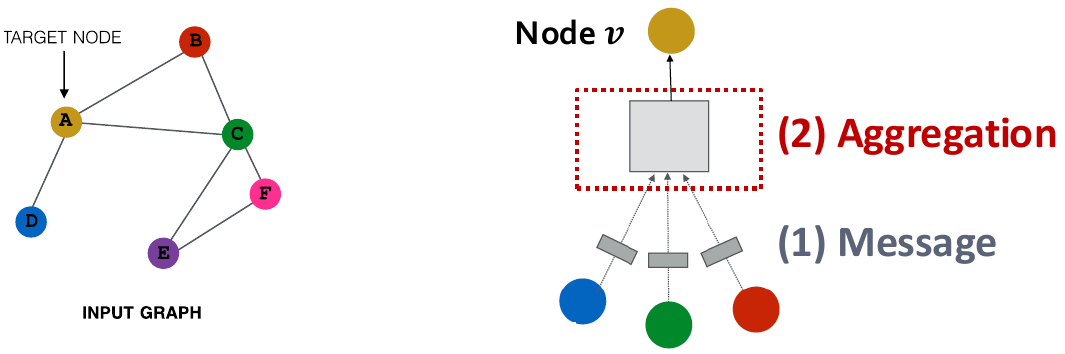
\includegraphics[
                    width=0.5\linewidth,
                    trim=0pt 0pt 0pt 0pt, % trim: left bottom right top
                    clip
                ]{../images/message_passing_aggregation.png}
                \caption{Aggregation function.}
                \source{\url{https://web.stanford.edu/class/cs224w/}.}
                % \label{fig:my_image}
            \end{figure}

            \begin{note}
                {Introduce your self}
            \end{note}
        \end{frame}

        \begin{frame}{General GNN layer}
            \alert{Node-level form:}

            \begin{equation}
                % \mathbf{h}_{v}^{(l)} = \sigma\!\left(\mathbf{W}^{(l)}\cdot \text{AGGREGATE}\!\left(\left\{\mathbf{h}_{u}^{(l-1)},\; u\in \mathcal{N} (v)\right\},\, \mathbf{h}_{v}^{(l-1)}\right)\right)
                % \mathbf{h}_{v}^{(l)} = \sigma\!\left(\mathbf{W}^{(l)}\cdot \text{AGGREGATE}\!\left(\left\{\mathbf{h}_{u}^{(l-1)} \mid u\in \mathcal{N} (v) \cup \{v\}\right\}\right)\right)
                % \mathbf{h}_{v}^{(l)} = \sigma\!\left(\mathbf{W}^{(l)} \text{AGGREGATE}^{(l)}\!\left(\left\{\text{MESSAGE}^{(l)}\left(h_u^{(l-1)} \mid u\in \mathcal{N} (v) \cup \{v\}\right)\right\}\right)\right)
                h_{u}^{(l)} = \sigma\!\left(\text{AGGREGATE}^{(l)}\!\left(\left\{\text{MESSAGE}^{(l)}\left(h_v^{(l-1)}\right) \mid v \in \mathcal{N} (u) \cup \{u\}\right\}\right)\right)
                % \label{eq:equation1}
            \end{equation}

            \begin{equation}
                % h_{v}^{(l)} = \sigma\!\left(W^{(l)} \cdot \text{AGGREGATE}^{(l)}\left(\left\{ h_{u}^{(l - 1)} \mid u \in \mathcal{N}(v) \cup \{v\}\right\}\right)\right)
                h_{u}^{(l)} = \sigma\!\left(\sum_{v \in \mathcal{N}(u) \cup \{u\}}h_v^{(l-1)}W^{(l)}\right)
                % \label{eq:equation1}
            \end{equation}

            \alert{Matrix form:}

            \begin{equation}
                % H^{(l)} = \sigma\left(\hat{A}\cdot\mathrm{MSG}^{(l)}\left(H^{(l-1)}\right)\cdot W^{(l)}\right)
                H^{(l)} = \sigma\left(\tilde{A}H^{(l-1)} W^{(l)}\right)
                % \label{eq:equation1}
            \end{equation}

            Where:
            \begin{itemize}
                \item $\text{MESSAGE}^{(l)}\left(h_v^{(l-1)}\right) \quad \longrightarrow \quad H^{(l-1)}W^{(l)}$
                \item $\text{AGGREGATE}^{(l)}(\cdot) \quad \longrightarrow \quad \tilde{A}(\cdot), \;\; \tilde{A} = A + I$
            \end{itemize}

            \begin{note}
                {Introduce your self}
            \end{note}
        \end{frame}

        \begin{frame}{Deeper GNNs}
            \begin{alertblock}{Oversmoothing problem}
                As the number of layers $L$ grows, each node aggregates information from an increasingly larger portion of the graph. This causes all node embeddings $h_v^{(L)}$ to become too similar to each other, losing the ability to distinguish between nodes.
            \end{alertblock}

            \begin{figure}[htp!]
                \centering
                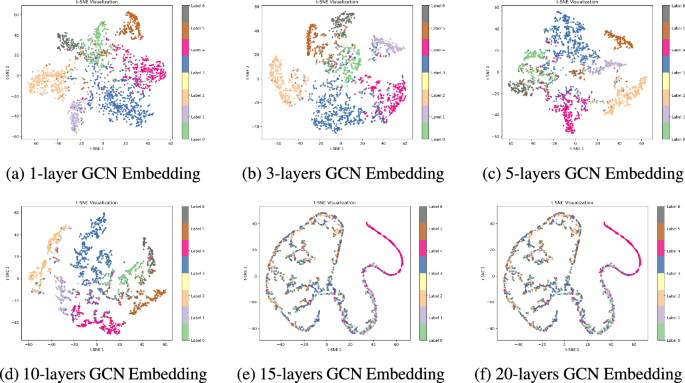
\includegraphics[
                    width=0.5\linewidth,
                    trim=0pt 0pt 0pt 0pt, % trim: left bottom right top
                    clip
                ]{../images/GNN_oversmoting_example.png}
                \caption{Oversmoothing examples.}
                \source{\url{https://link.springer.com/article/10.1007/s10115-025-02548-6}}
                % \label{fig:my_image}
            \end{figure}

            \begin{note}
                {Introduce your self}
            \end{note}
        \end{frame}

        \begin{frame}{Splitting graphs}
            \begin{itemize}
                \item \alert{Transductive settings}: The complete input graph $G = (V, E)$ is observed during training, validation, and testing, with only the node labels differing across the dataset splits.
                \item \alert{Inductive settings}: The graph $G = (V, E)$ is partitioned by removing the edges between the different components, resulting in multiple disconnected graphs.
            \end{itemize}

            \begin{figure}
                \centering
                \begin{subfigure}{0.3\textwidth}
                    \centering
                    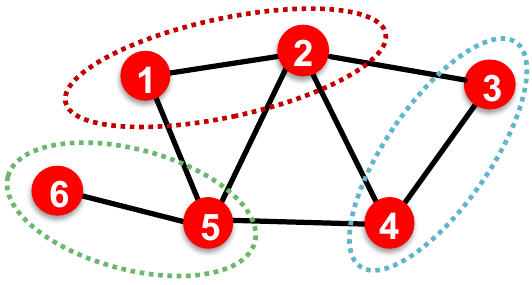
\includegraphics[
                        width=\linewidth,
                        trim=0pt 0pt 0pt 0pt, % trim: left bottom right top
                        clip
                    ]{../images/GNN_split_transductive.png}
                    \caption{Transductive.}
                    % \source{Author, 2024.}
                \end{subfigure}
                % \hfill
                \hspace{1cm}
                \begin{subfigure}{0.3\textwidth}
                    \centering
                    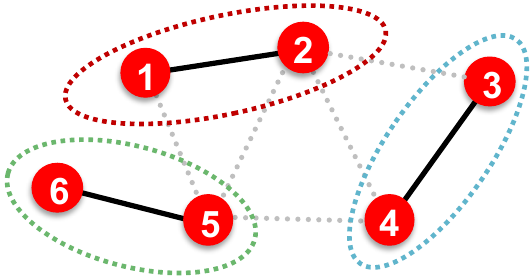
\includegraphics[
                        width=\linewidth,
                        trim=0pt 0pt 0pt 0pt, % trim: left bottom right top
                        clip
                    ]{../images/GNN_split_inductive.png}
                    \caption{inductive.}
                    % \source{Author, 2024.}
                \end{subfigure}
                \caption{Splitting graphs. Red: training, blue: validation, and green: test.}
                \source{\url{https://web.stanford.edu/class/cs224w/}.}
                % \label{fig:my_image}
            \end{figure}

            \begin{note}
                {Introduce your self}
            \end{note}
        \end{frame}

        \begin{frame}{GNN training pipeline}
            \begin{figure}[htp!]
                \centering
                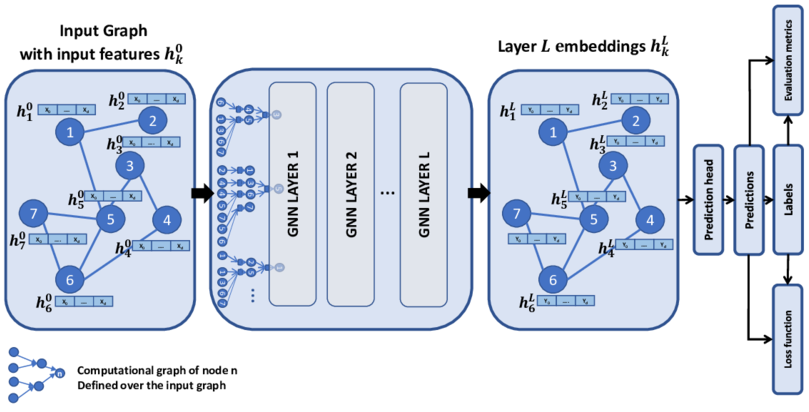
\includegraphics[
                    width=0.65\linewidth,
                    trim=0pt 0pt 0pt 0pt, % trim: left bottom right top
                    clip
                ]{../images/GNN_traing_pipeline.png}
                \caption{GNN training pipeline.}
                \source{\url{https://www.researchgate.net/figure/GNN-training-pipeline-illustration_fig1_366001542}}
                % \label{fig:my_image}
            \end{figure}

            \begin{equation}
                \scriptsize
                % \underbrace{G = (V, E, X)}_{\text{input}} \xrightarrow{\text{GNN layers}} \underbrace{H^{(L)}}_{\text{node embeddings}} \xrightarrow{\text{prediction head}} \underbrace{\hat{Y}}_{\text{predictions}} \xrightarrow{\text{loss}} \underbrace{\mathcal{L}}_{\text{backprop}} \xrightarrow{\text{update}} \underbrace{W^{(1)},\dots,W^{(L)}}_{\text{learned weights}}
                % \underbrace{G=(V,E,X)}_{\text{input graph}} \xrightarrow{\text{GNN layers}} \underbrace{Z = H^{(L)}}_{\text{node embeddings}} \xrightarrow{W_{\text{pred}}} \underbrace{\hat{Y}}_{\text{predictions}}
                \underbrace{G=(V,E,X)}_{\text{input graph}} \xrightarrow{\text{GNNs}} \underbrace{Z = H^{(L)}}_{\text{node embeddings}} \xrightarrow{f_{\theta}} \underbrace{\hat{Y}}_{\text{predictions}}
                % W_out, W_pred, MLP(.), f_{theta}(.)
                % \label{eq:equation1}
            \end{equation}

            \begin{note}
                {Introduce your self}
            \end{note}
        \end{frame}

    \subsection{More about embeddings}
        \begin{frame}{More about embeddings}
            \begin{figure}[htp!]
                \centering
                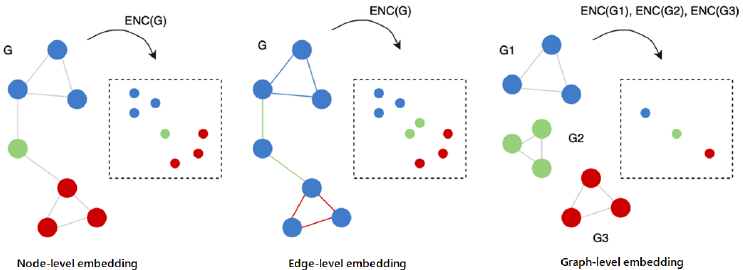
\includegraphics[
                    width=0.9\linewidth,
                    trim=0pt 0pt 0pt 0pt, % trim: left bottom right top
                    clip
                ]{../images/more_embeddings.png}
                \caption{Visual representation of the three different levels of granularity in graphs.}
                % \source{Author, 2024.} grover2016node2vec
                % \label{fig:my_image}
            \end{figure}

            \begin{note}
                {Introduce your self}
            \end{note}
        \end{frame}

        \begin{frame}{Edge-level embeddings}
            % An \textit{edge embedding} is formally defined as a function $f: E \rightarrow \mathbb{R}^{d}$ that maps each edge of the graph $G = (V, E)$ to a low-dimensional vector representation, preserving relevant structural properties of the graph. \newline
            % The resulting set $Z^{(e)} = \{z_{uv} = f(u, v) \in \mathbb{R}^{d} \mid (u, v) \in E\}$, where each $z_{uv}$ is called an \alert{edge embedding}, is computed for each pair of nodes $(u, v) \in E$ from their corresponding node embeddings $z_u, z_v \in \mathbb{R}^{d}$ using an aggregation operator $\phi$, such that $z_{uv} = \phi(z_u, z_v)$.

            It is a function $f: E \rightarrow \mathbb{R}^{d}$ that maps each edge of the graph $G = (V, E)$ to a low-dimensional vector, where $z_{uv} = \phi(z_u, z_v) \in \mathbb{R}^{d} \: \forall \: (u, v) \in E$ is called an \alertplain{edge embedding}, computed from the node embeddings $z_u, z_v$ via an aggregation operator $\phi$. \newline %, for each pair $(u, v) \in E$. \newline

            \alert{Operators:}
            \begin{description}
                \item [Concatenate:] $z_{uv} = z_u \oplus z_v$
                \item [Sum:] $z_{uv} = z_u + z_j$
                \item [Average:] $z_{uv} = \frac{z_u + z_v}{2}$
                \item [Hadamard:] $z_{uv} = z_u \ast z_v$
                \item [Weighted-L1:] $z_{uv} = \vert z_u - z_v\vert$
                \item [Weighted-L2:] $z_{uv} = \vert z_u - z_v\vert^2$
            \end{description}

            \begin{note}
                {Introduce your self}
            \end{note}
        \end{frame}

        \begin{frame}{Application of aggregation operators}
            \begin{figure}[htp!]
                \centering
                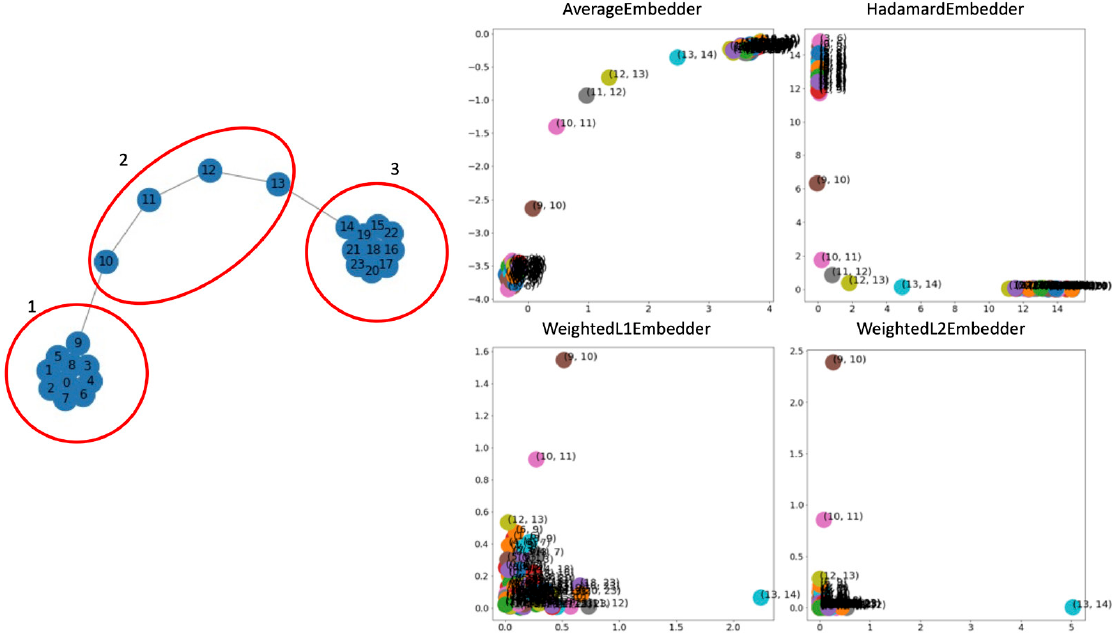
\includegraphics[
                    width=0.78\linewidth,
                    trim=0pt 0pt 0pt 0pt, % trim: left bottom right top
                    clip
                ]{../images/edge_embeddings_operators.png}
                \caption{Comparison of aggregation operators for edge embedding.}
                % \source{Author, 2024.} grover2016node2vec
                % \label{fig:my_image}
            \end{figure}

            \begin{note}
                {Introduce your self}
            \end{note}
        \end{frame}

        \begin{frame}{Graph-level embeddings}
            % A \textit{graph-level embedding} is a function $f: G \rightarrow \mathbb{R}^{d}$ that maps the entire graph $G = (V, E)$ to a single low-dimensional vector representation. \newline
            % The resulting vector $z_G = f(G) \in \mathbb{R}^{d}$ is called a \alert{graph embedding}, and is computed by aggregating the node embeddings $Z = \{z_1, z_2, \ldots, z_{|V|}\}$, $z_i \in \mathbb{R}^{d}$, through a \textit{global pooling} operator $\phi$, also known as \textit{graph-level readout}, such that $z_G = \phi(z_1, z_2, \ldots, z_{|V|})$.
            It is a function $f: G \rightarrow \mathbb{R}^{d}$ that maps the entire graph $G = (V, E)$ to a single vector $z_G = \phi(z_1, z_2, \ldots, z_{|V|}) \in \mathbb{R}^{d}$, called \alertplain{graph embedding}, obtained by aggregating the node embeddings $z_i \in \mathbb{R}^{d}$ through a \textit{global pooling} or graph-level \textit{readout} operator $\phi$. \newline

            \alert{Operators:}
            \begin{description}
                \item [Mean global pooling:] $z_G = \frac{1}{|V|} \sum_{i=1}^{|V|}z_{i}$
                \item [Max global pooling:] $z_G = \max_{i=1}^{|V|}(z_{i})$
                \item [Sum global pooling:] $z_G = \sum_{i=1}^{|V|}z_{i}$
            \end{description}

            \begin{note}
                {Introduce your self}
            \end{note}
        \end{frame}

        \begin{frame}{Example}
            \begin{columns}[t] % Option "c" centers vertically, while "t" aligns to the top.
                \begin{column}{0.5\textwidth}
                    Given the graph $G = (V, E)$ and the node embedding matrix $Z$, compute the edge-level and graph-level embeddings: % the following node embedding matrix $Z \in \mathbb{R}^{5 \times 3}$:

                    \[
                        \footnotesize
                        Z =
                        \begin{bmatrix}
                        0.5 & 0.2 & 0.8 \\
                        0.1 & 0.9 & 0.4 \\
                        0.6 & 0.3 & 0.7 \\
                        0.2 & 0.5 & 0.1 \\
                        0.8 & 0.4 & 0.6
                        \end{bmatrix}
                    \]

                    % where each row $z_i \in \mathbb{R}^{3}$ represents the node embedding of node $i$.

                    \begin{figure}[htp!]
                        \centering
                        
\includegraphics[
                            width=0.425\linewidth,
                            trim=0pt 0pt 0pt 0pt, % trim: left bottom right top
                            clip
                        ]{../images/union.pdf}
                        \caption{Graph $G$.}
                        % \source{Author, 2024.}
                        % \label{fig:my_image}
                    \end{figure}
                \end{column}
                \begin{column}{0.5\textwidth}

                \end{column}
            \end{columns}
            
            \begin{note}
                {Introduce your self}
            \end{note}
        \end{frame}

        \begin{frame}{Graph learning tasks}
            \begin{figure}[htp!]
                \centering
                
\includegraphics[
                    width=1.0\linewidth,
                    trim=0pt 0pt 0pt 0pt, % trim: left bottom right top
                    clip
                ]{../images/graph_learning_tasks.pdf}
                \caption{Overview of graph learning tasks.}
                % \source{\url{https://www.researchgate.net/figure/Pipeline-for-applying-graph-embedding-methods-to-biomedical-tasks-Low-dimensional-node_fig1_336279199}}
                % \label{fig:my_image}
            \end{figure}

            \begin{note}
                {Introduce your self}
            \end{note}
        \end{frame}

        \begin{frame}{Example of graph learning tasks}
            \begin{figure}[htp!]
                \centering
                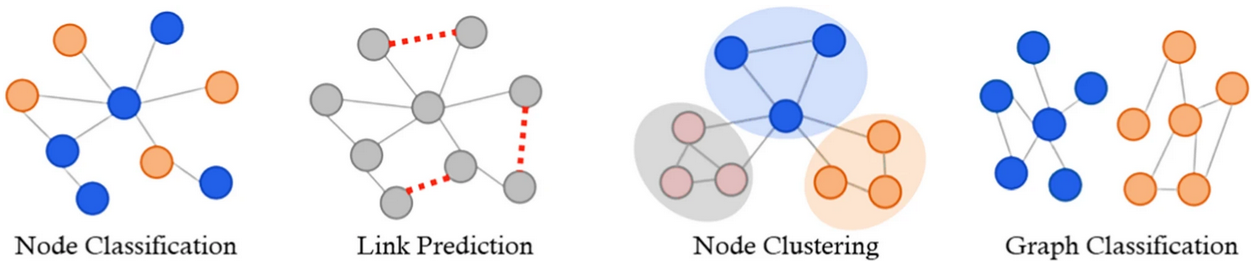
\includegraphics[
                    width=0.8\linewidth,
                    trim=0pt 0pt 0pt 0pt, % trim: left bottom right top
                    clip
                ]{../images/GNNS_task.png}
                \caption{Common tasks.}
                \source{\url{https://link.springer.com/article/10.1007/s10791-025-09569-3}}
                % \label{fig:my_image}
            \end{figure}

            \begin{note}
                {Introduce your self}
            \end{note}
        \end{frame}

        \begin{frame}{Variants of GNNs}
            \begin{itemize}
                \item Graph Convolutional Networks (GCN) % \cite{kipf2016semi}
                % \item Graph Recurrent Networks (GRN)
                \item Graph Attention Networks (GAT) % \cite{velickovic2017graph}
                \item Graph Isomorphism Networks (GIN) % \cite{xu2018powerful}
                
                \item Variational Graph Auto-Eencoders (VGAE) % \cite{kipf2016variational}
                \item Deep Graph Infomax (DGI) % \cite{velivckovic2018deep}
                \item Adversarially Regularized Variational Graph Autoencoder (ARVGA) % \cite{pan2018adversarially}
                \item Linear Graph Variational Autoencoder (LGVAE) % \cite{salha2021simple}
                \item ...
            \end{itemize}
        \end{frame}

        \begin{frame}{Recap: General GNN layer}
            \alert{Node-level form:}

            \begin{equation}
                % \mathbf{h}_{v}^{(l)} = \sigma\!\left(\mathbf{W}^{(l)}\cdot \text{AGGREGATE}\!\left(\left\{\mathbf{h}_{u}^{(l-1)},\; u\in \mathcal{N} (v)\right\},\, \mathbf{h}_{v}^{(l-1)}\right)\right)
                % \mathbf{h}_{v}^{(l)} = \sigma\!\left(\mathbf{W}^{(l)}\cdot \text{AGGREGATE}\!\left(\left\{\mathbf{h}_{u}^{(l-1)} \mid u\in \mathcal{N} (v) \cup \{v\}\right\}\right)\right)
                % \mathbf{h}_{v}^{(l)} = \sigma\!\left(\mathbf{W}^{(l)} \text{AGGREGATE}^{(l)}\!\left(\left\{\text{MESSAGE}^{(l)}\left(h_u^{(l-1)} \mid u\in \mathcal{N} (v) \cup \{v\}\right)\right\}\right)\right)
                h_{u}^{(l)} = \sigma\!\left(\text{AGGREGATE}^{(l)}\!\left(\left\{\text{MESSAGE}^{(l)}\left(h_v^{(l-1)}\right) \mid v \in \mathcal{N} (u) \cup \{u\}\right\}\right)\right)
                % \label{eq:equation1}
            \end{equation}

            \begin{equation}
                % h_{v}^{(l)} = \sigma\!\left(W^{(l)} \cdot \text{AGGREGATE}^{(l)}\left(\left\{ h_{u}^{(l - 1)} \mid u \in \mathcal{N}(v) \cup \{v\}\right\}\right)\right)
                h_{u}^{(l)} = \sigma\!\left(\sum_{v \in \mathcal{N}(u) \cup \{u\}}h_v^{(l-1)}W^{(l)}\right)
                % \label{eq:equation1}
            \end{equation}

            \alert{Matrix form:}

            \begin{equation}
                % H^{(l)} = \sigma\left(\hat{A}\cdot\mathrm{MSG}^{(l)}\left(H^{(l-1)}\right)\cdot W^{(l)}\right)
                H^{(l)} = \sigma\left(\tilde{A}H^{(l-1)} W^{(l)}\right)
                % \label{eq:equation1}
            \end{equation}

            Where:
            \begin{itemize}
                \item $\text{MESSAGE}^{(l)}\left(h_v^{(l-1)}\right) \quad \longrightarrow \quad H^{(l-1)}W^{(l)}$
                \item $\text{AGGREGATE}^{(l)}(\cdot) \quad \longrightarrow \quad \tilde{A}(\cdot), \;\; \tilde{A} = A + I$
            \end{itemize}

            \begin{note}
                {Introduce your self}
            \end{note}
        \end{frame}

        \begin{frame}{Graph Convolutional Networks (GCNs)}
            % https://dl.acm.org/doi/pdf/10.1145/2623330.2623732
            \alert{GCN}: Semi-Supervised Classification with Graph Convolutional Networks
            
            {\scriptsize (Kipf, T. N., \& Welling, M., 2016)}

            \begin{figure}[htp!]
                \centering
                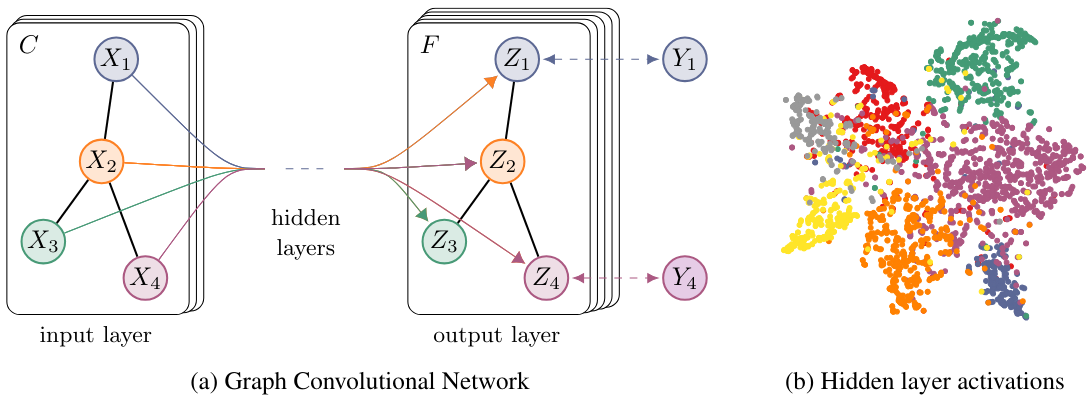
\includegraphics[
                    width=0.9\linewidth,
                    trim=0pt 0pt 0pt 0pt, % trim: left bottom right top
                    clip
                ]{../images/CGN_model.png}
                \caption{GCN workflow.} % Schematic depiction of multi-layer Graph Convolutional Network (GCN) for semi-supervised learning with C input channels and F feature maps in the output layer. The graph structure (edges shown as black lines) is shared over layers, labels are denoted by Yi. Right: t-SNE (Maaten & Hinton, 2008) visualization of hidden layer activations of a two-layer GCN trained on the Cora dataset (Sen et al., 2008) using 5% of labels. Colors denote document class
                \source{\url{https://arxiv.org/pdf/1609.02907}}
                % \label{fig:my_image}
            \end{figure}

            \begin{note}
                {Introduce your self}
            \end{note}
        \end{frame}

        \begin{frame}{Graph Convolutional Networks (GCNs)}
            For each node $u$ the embedding at layer $l$ is computed by aggregating the normalized messages from all neighbors $v \in \mathcal{N}(u) \cup \{u\}$. % \newline

            \alert{Node-level form:}
            \begin{equation}
                % h_v^{(l)} = \sigma\left(\sum_{u \in \mathcal{N}(v) \cup \{v\}} \frac{1}{\sqrt{\deg(v)\deg(u)}}\, h_u^{(l-1)}W^{(l)}\right)
                h_u^{(l)} = \sigma\left(\sum_{v \in \mathcal{N}(u) \cup \{u\}} \frac{1}{\sqrt{|\mathcal{N}(u) \cup \{u\}| \, |\mathcal{N}(v) \cup \{v\}|}}\, h_v^{(l-1)} W^{(l)}\right)
                % \label{eq:equation1}
            \end{equation}

            \alert{Matrix form:}
            \begin{equation}
                % H^{(l)} = \sigma\left(\hat{A}H^{(l-1)} W^{(l)}\right)
                H^{(l)} = \sigma\left(\tilde{D}^{-\frac{1}{2}}\tilde{A}\tilde{D}^{-\frac{1}{2}}H^{(l-1)} W^{(l)}\right)
                % \label{eq:equation1}
            \end{equation}

            Where:
            \begin{itemize}
                % \item Normalized adjacency matrix: $\hat{A} = \tilde{D}^{-\frac{1}{2}}\tilde{A}\tilde{D}^{-\frac{1}{2}}$
                \item Adjacency matrix with self-connections: $\tilde{A} = A + I$
                \item Degree matrix of $\tilde{A}$: $\tilde{D}_{uu} = \sum_v \tilde{A}_{uv}$
                \item Normalized adjacency matrix: $\hat{A} = \tilde{D}^{-\frac{1}{2}}\tilde{A}\tilde{D}^{-\frac{1}{2}}$
                \item Node embedding matrix at layer $l-1$: $H^{(l-1)} \in \mathbb{R}^{|V| \times d}$
                \item Learnable weight matrix: $W^{(l)} \in \mathbb{R}^{d \times d'}$
                % \item Initialization with node features: $H^{(0)} = X$
            \end{itemize}

            \begin{note}
                {Introduce your self}
            \end{note}
        \end{frame}

        \begin{frame}{Example}
            \begin{columns}[t] % Option "c" centers vertically, while "t" aligns to the top.
                \begin{column}{0.5\textwidth}
                    Given the graph $G = (V, E)$, the node feature matrix $X$, $L = 1$, $W$, and $\text{ReLU}(\cdot)$. Compute the node embedding matrix $Z$:

                    \[
                        \footnotesize
                        X = 
                        \begin{bmatrix} 
                            1 & 0 & 1 \\ 
                            0 & 1 & 0 \\ 
                            1 & 1 & 0 \\ 
                            0 & 1 & 1 \\ 
                            1 & 0 & 1 
                        \end{bmatrix}, \quad 
                        W = 
                        \begin{bmatrix} 
                            1 & -1 & 0 \\ 
                            2 & 0 & 1 \\ 
                            -1 & 1 & 2 
                        \end{bmatrix}
                    \]
                    %\vspace{-0.6cm}
                    \begin{figure}[htp!]
                        \centering
                        
\includegraphics[
                            width=0.425\linewidth,
                            trim=0pt 0pt 0pt 0pt, % trim: left bottom right top
                            clip
                        ]{../images/union.pdf}
                        \caption{Graph $G$.}
                        % \source{Author, 2024.}
                        % \label{fig:my_image}
                    \end{figure}
                \end{column}
                \begin{column}{0.5\textwidth}

                \end{column}
            \end{columns}
            
            \begin{note}
                {Introduce your self}
            \end{note}
        \end{frame}

        \begin{frame}{Node classification task}
            \begin{figure}
                \centering
                \begin{subfigure}{0.241\textwidth}
                    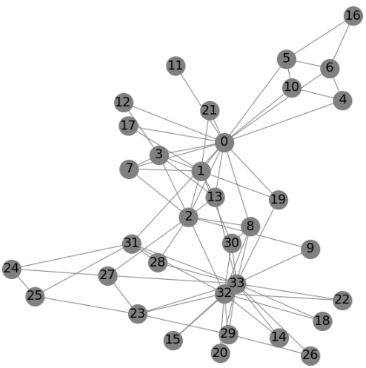
\includegraphics[width=1.0\textwidth]{../images/input_graph.png}
                    \caption{\scriptsize Input graph.}
                    %%% \label{fig:input_graph_}
                \end{subfigure}
                \hfill
                \begin{subfigure}{0.241\textwidth}
                    \centering
                % \includegraphics{}
                \animategraphics[width=1.3\textwidth, loop, autoplay]
                {5} % frame rate
                {../images/train_gcn/download_} % path to figures
                {0} % start index
                {149} % end index
                \caption{Train GCN.}
                %%% \label{fig:my_label}
                \end{subfigure}
                \hfill
                \begin{subfigure}{0.241\textwidth}
                    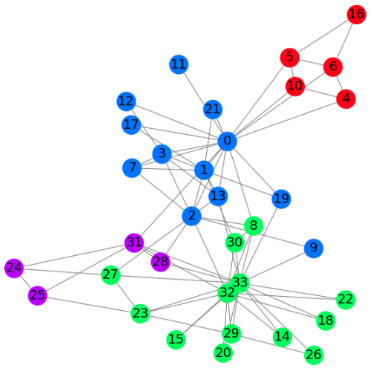
\includegraphics[width=\textwidth]{../images/output_graph.png}
                    \caption{\scriptsize Output graph.}
                    %%% \label{fig:output_graph}
                \end{subfigure}
                \caption{\scriptsize GCN to node classification.}
                %%% \label{fig:node_classification}
            \end{figure}
        \end{frame}

        \begin{frame}{Practical example: GCN to node classificationn}
            \begin{itemize}
                \item Install requirements
                    \begin{itemize}
                        \item \texttt{Python}
                        \item \texttt{Pandas} 
                        % \item \texttt{NumPy}
                        \item \texttt{PyTorch Geometric}
                        \item \texttt{NetworkX}
                        \item \texttt{Matplotlib} / \texttt{Plotly} / \texttt{Seaborn}
                        \item \texttt{Scikit-learn}
                    \end{itemize}
                \item Topics 
                    \begin{itemize}
                        \item Data preparation
                        \item Select model
                        \item Train model (for node classification)
                        \item Evaluate model
                        \item Embeddings visualization
                    \end{itemize}
                \item Lab
                    \begin{itemize}
                        \item \href{https://drive.google.com/file/d/1YVt5cgHTjLYzOOe-ihFGGy7ZjAdk-v5G/view?usp=sharing}{
                                \beamergotobutton{\faGoogle\ Open in Google Colab}
                            }
                    \end{itemize}
            \end{itemize}
            
            \begin{note}
                {Write your notes here}
            \end{note}
        \end{frame}

% Applications
\section{Applications}
    \begin{frame}{Applications}
        \begin{multicols}{2}
            \begin{itemize}
                \item Computer vision
                \item Natural language processing
                \item Recommender systems
                \item Program analysis
                \item Knowledge graphs
                \item Bioinformatics
                \item Chemistry
                \item Biology
                \item Physic
                \item Anomaly detection
                \item Urban intelligence
                \item Financial transaction
                \item ...
            \end{itemize}
        \end{multicols}          
    \end{frame}

    \begin{frame}{Application in computer vision}
        \alert{SuperGlue}: Learning Feature Matching with Graph Neural Networks %  \cite{sarlin2020superglue}.
        
        {\scriptsize (Sarlin, P. E., DeTone, D., Malisiewicz, T., \& Rabinovich, A., 2020)}
        
        \begin{figure}[ht!]
            \centering
            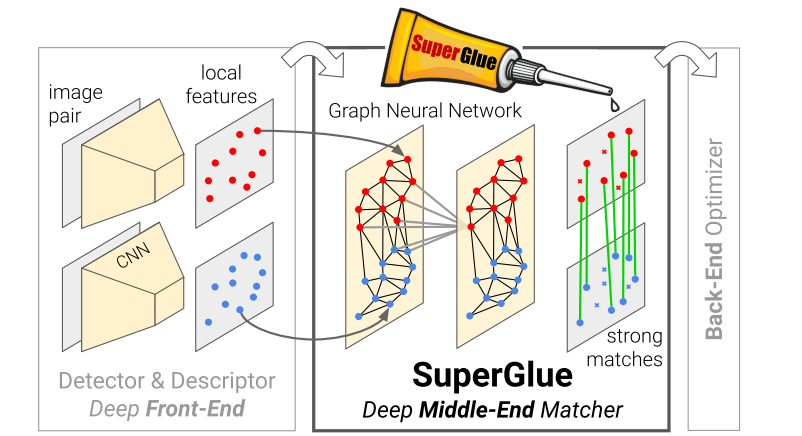
\includegraphics[width=0.7\linewidth]{../images/super_glue.png}
            \caption{SuperGlue scheme.}
        \end{figure}
    \end{frame}
    
    \begin{frame}{SuperGlue in action}
        \begin{figure}
            \centering
            % \includegraphics{}
            \animategraphics[width=\textwidth, loop, autoplay]
            {5} % frame rate
            {../images/imd/freiburg_matches-} % path to figures
            {0} % start index
            {15} % end index
            \caption{Matching example (indoor).}
            %%% \label{fig:app_superglue}
        \end{figure}
    \end{frame}

    \begin{frame}{SuperGlue in action}
        \begin{figure}[ht!]
            \centering
            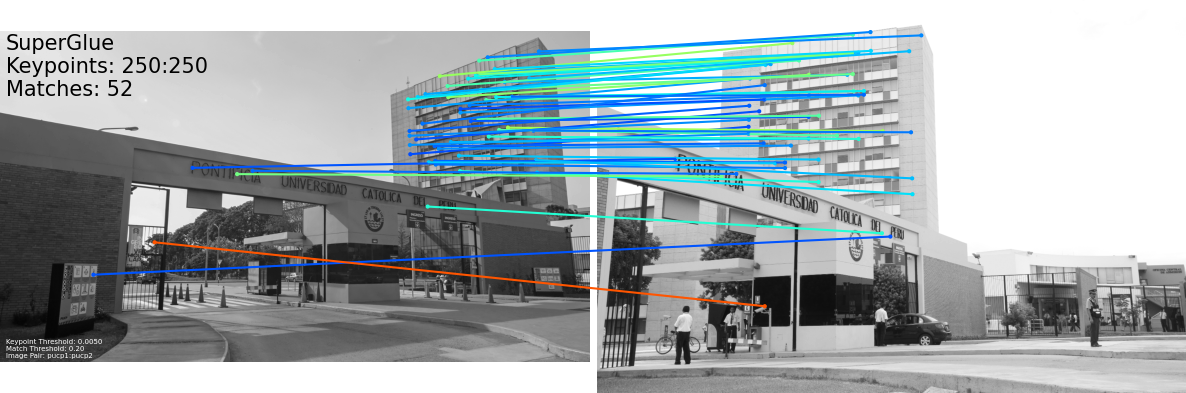
\includegraphics[width=1.0\linewidth]{../images/pucp1_pucp2_matches.png}
            \caption{Matching images.}
        \end{figure}
    \end{frame}

    \begin{frame}{Application in urban intelligence}
        \alert{Spatio-Temporal Graph Convolutional Networks}: A Deep Learning Framework for Traffic Forecasting % \cite{yu2017spatio}.

        {\scriptsize (Yu, B., Yin, H., \& Zhu, Z., 2017)}
        
        \begin{figure}[ht!]
            \centering
            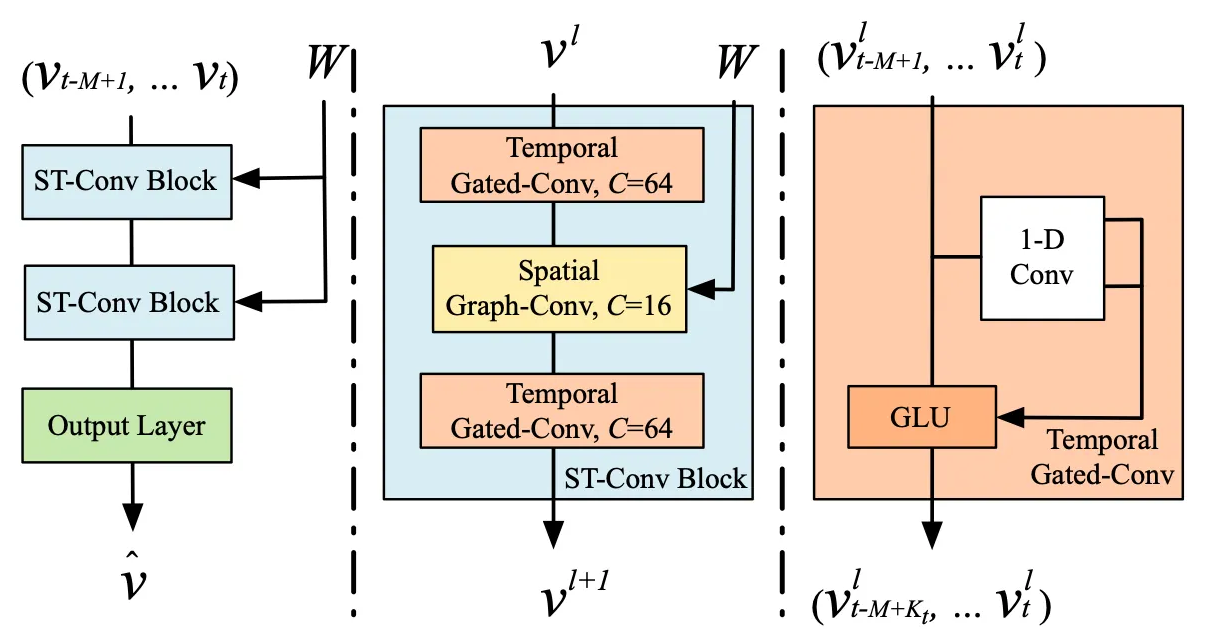
\includegraphics[width=0.65\linewidth]{../images/stgcn_model.png}
            \caption{STGCN scheme.}
        \end{figure}
    \end{frame}
    
    \begin{frame}{STGCN in action}
        \begin{figure}
            \centering
            % \includegraphics{}
            \animategraphics[width=0.65\textwidth, loop, autoplay]
            {15} % frame rate
            {../images/traffic/c389b48c98f34cce898d9c1baa2ed346LTsk9cwQTrdumRQT-} % path to figures
            {0} % start index
            {232} % end index
            \caption{Visualization of traffic}
            \source{\url{https://medium.com/stanford-cs224w/predicting-evolution-of-dynamic-graphs-7688eca1daf8}}
            % \label{fig:my_image}
        \end{figure}
    \end{frame}

    \begin{frame}{Application in physic}
        Learning to Simulate Complex Physics with Graph Networks % \cite{sanchez2020learning}.

        {\scriptsize (Sanchez-Gonzalez, A., Godwin, J., Pfaff, T., Ying, R., Leskovec, J., \& Battaglia, P., 2020)}
        
        \begin{figure}[ht!]
            \centering
            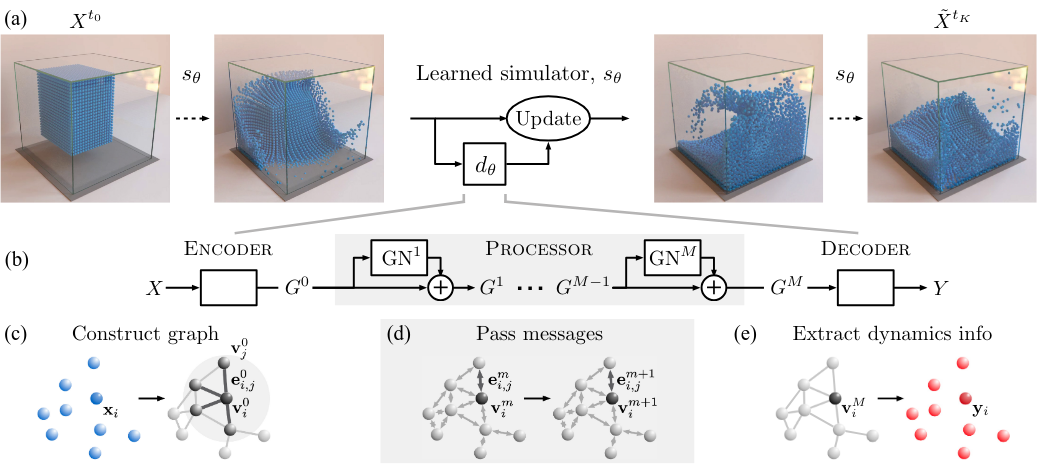
\includegraphics[width=0.85\linewidth]{../images/gns.png}
            \caption{GNS scheme.}
        \end{figure}
    \end{frame}
    
    \begin{frame}{GNS in action}
        \begin{figure}
            \centering
            % \includegraphics{}
            \animategraphics[width=0.85\textwidth, loop, autoplay]
            {10} % frame rate
            {../images/physics/96e5eb9cda094a5dacfe00a168965330KkJlbebmdYjuPPbO-} % path to figures
            {0} % start index
            {149} % end index
            \caption{Simulating complex physics.}
            \source{\url{https://medium.com/stanford-cs224w/simulating-complex-physics-with-graph-networks-step-by-step-177354cb9b05}}
            % \label{fig:my_image}
        \end{figure}
    \end{frame}

    \begin{frame}{Application in recommender systems}
        \alert{Uber Eats}

        \begin{figure}[htp!]
            \centering
            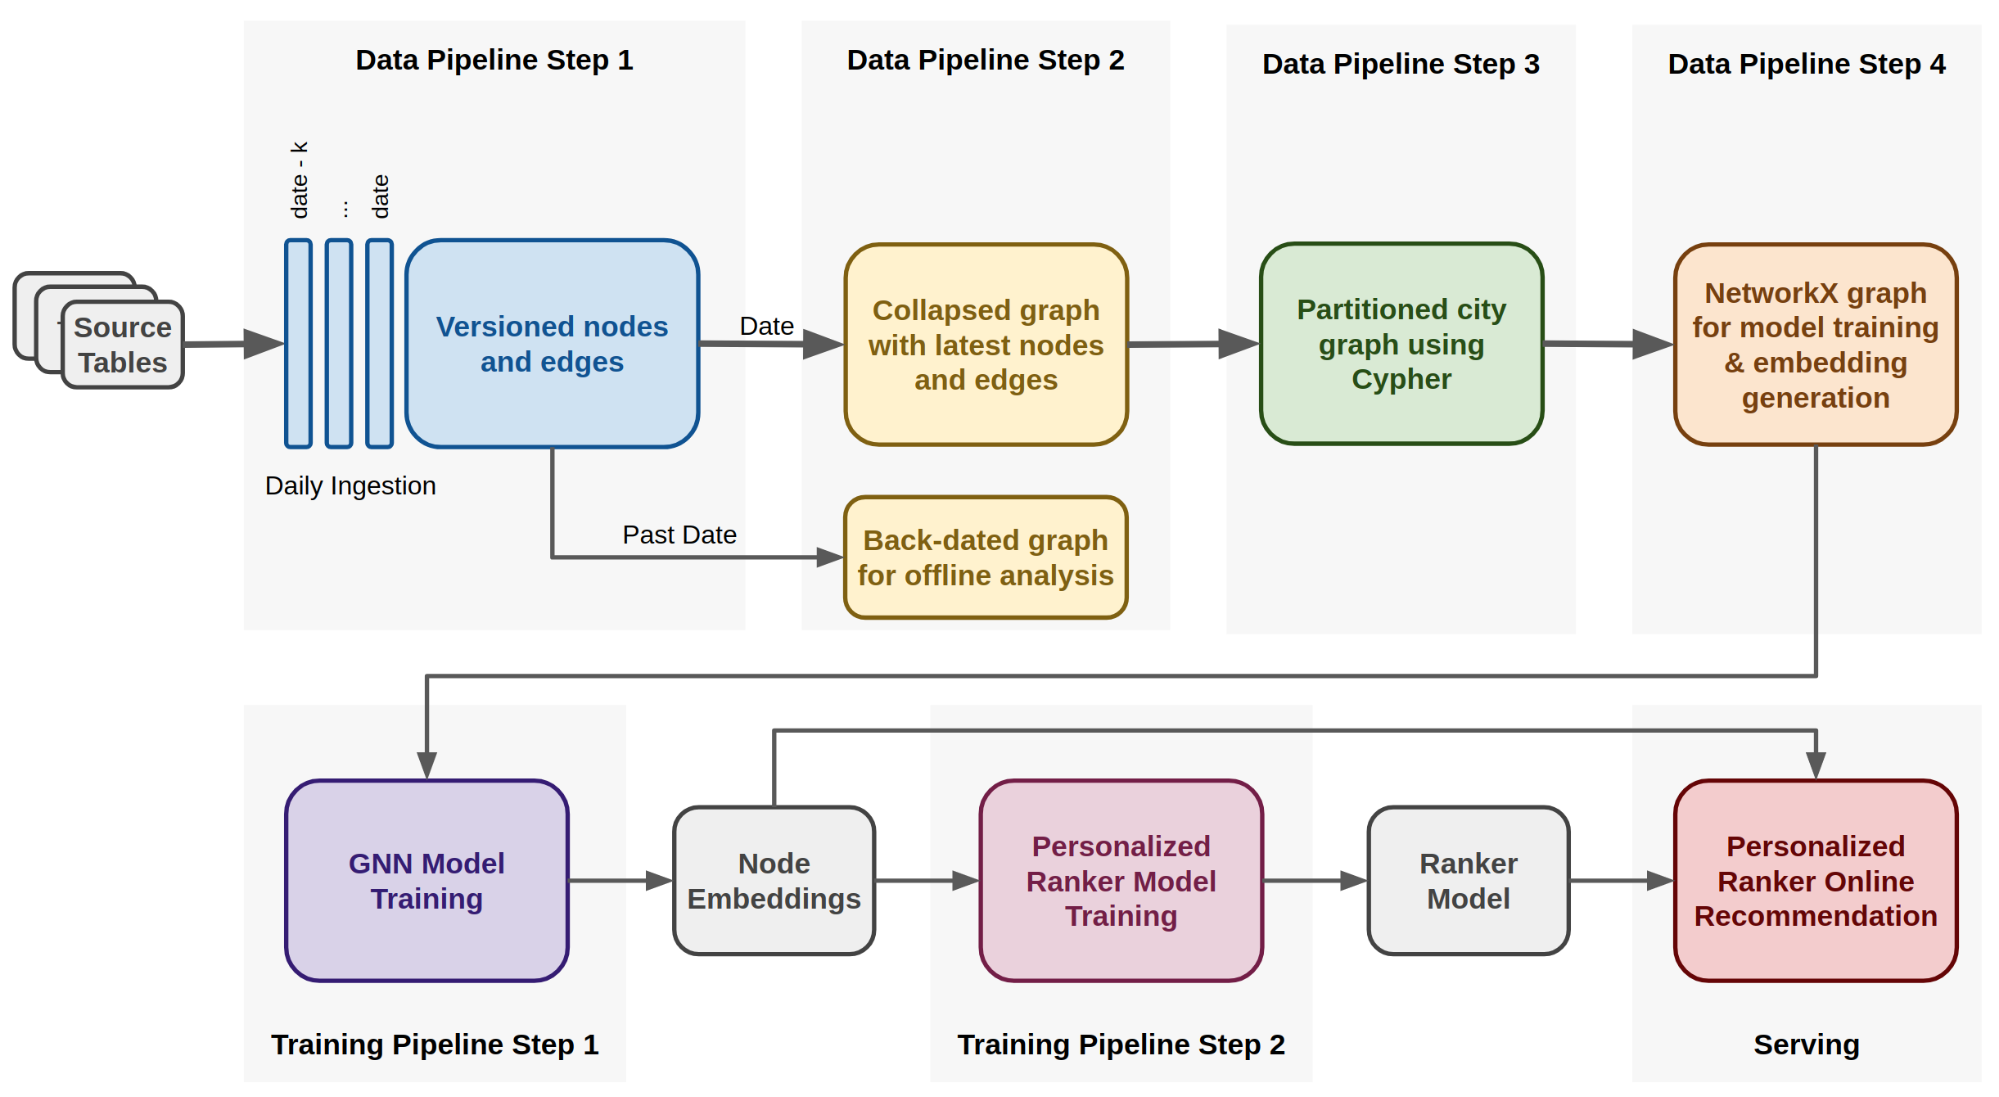
\includegraphics[
                width=0.7\linewidth,
                trim=0pt 0pt 0pt 0pt, % trim: left bottom right top
                clip
            ]{../images/uber_model.png}
            \caption{Pipeline Uber eats.}
            \source{\url{https://www.uber.com/en-CO/blog/uber-eats-graph-learning/}}
            % \label{fig:my_image}
        \end{figure}
    \end{frame}

    \begin{frame}{Uber Eats}
        \begin{figure}
            \centering
            % \includegraphics{}
            \animategraphics[width=0.25\textwidth, loop, autoplay]
            {5} % frame rate
            {../images/uber_eats/a733611516524151ebb9d28ad2c2ab68IaQ4dI3VB8Bs9CFt-} % path to figures
            {0} % start index
            {30} % end index
            \caption{Recommender systems app.}
            %%% \label{fig:app_ubereats}
        \end{figure}
    \end{frame}

% Resources
\section{Resources}
    \begin{frame}{Package, library, and framework}        
        \begin{figure}[ht!]
            \centering
            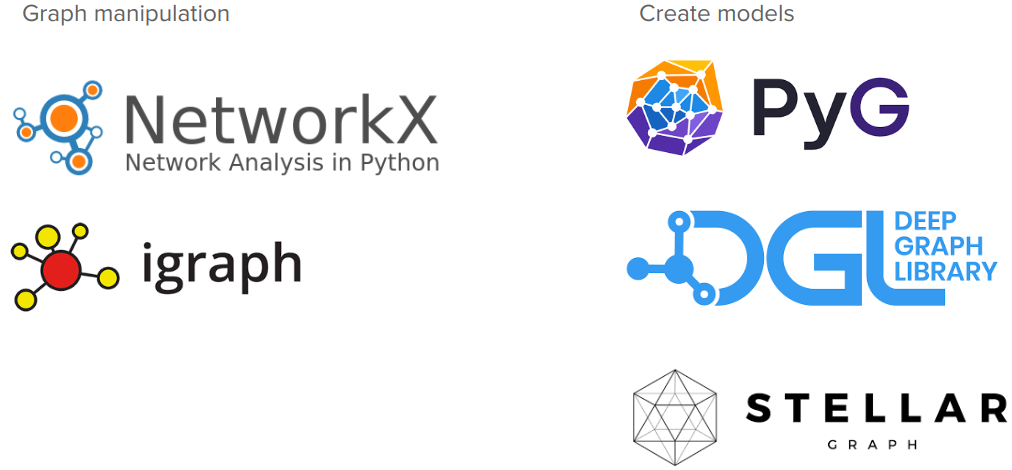
\includegraphics[width=0.9\linewidth]{../images/sources.png}
            \caption{Package, library, and framework.}
        \end{figure}               
    \end{frame}

    \begin{frame}{Books}
        \begin{figure}[ht!]
            \centering
            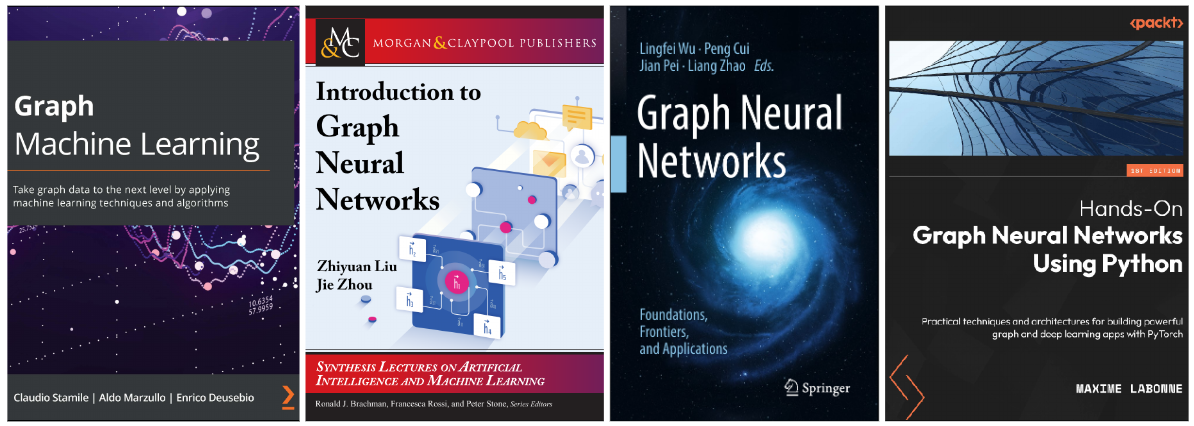
\includegraphics[width=1.0\linewidth]{../images/books_source.png}
            \caption{GNNs books.}
        \end{figure}               
    \end{frame}

    \begin{frame}{Further learning}
        \begin{itemize}
            \item Courses
            \begin{itemize}
                \item CS224W: Machine Learning with Graphs \\ (\url{http://web.stanford.edu/class/cs224w/})
            \end{itemize}
            \item Tutorials
            \begin{itemize}
                \item PyTorch Geometric: Introduction by Example \\ (\url{https://pytorch-geometric.readthedocs.io/en/latest/notes/introduction.html})
            \end{itemize}
            \item Conferences
            \begin{itemize}
                \item Learning on Graphs \\ (\url{https://logconference.org/})
            \end{itemize}
        \end{itemize}
    \end{frame}

\section*{References}    
    % Bibliography
    % \input{ref.bib}
    \begin{frame}[allowframebreaks]
        \footnotesize % use this command to resize
        % \bibliography{ref}
        % \bibliographystyle{unsrt}
        % \bibliographystyle{alpha}
        
        \begin{itemize}
            \item Erciyes, K. (2018). \textit{Guide to graph algorithms} % (pp. 15-35). Springer International Publishing.
            \item Yao Ma, Jiliang Tang. (2021). \textit{Deep Learning on Graphs}.
            \item Stamile C., Marzullo A., Deusebio E. (2021). \textit{Graph Machine Learning}.
            \item Wu, L., Cui, P., Pei, J., Zhao, L., \& Guo, X. (2022). \textit{Graph neural networks: foundation, frontiers and applications}. % In Proceedings of the 28th ACM SIGKDD conference on knowledge discovery and data mining (pp. 4840-4841).            
            % \item Knickerbocker D. (2023). \textit{Graph Network Science with Python}.
            \item Knickerbocker, D. (2023). \textit{Network Science with Python}. % Packt Publishing Ltd.
            \item Labonne, M. (2023). \textit{Hands-On Graph Neural Networks Using Python}.
            \item Broadwater, K., \& Stillman, N. (2025). \textit{Graph neural networks in action}. % Simon and Schuster.
        \end{itemize}
    \end{frame}

    \begin{frame}
        \begin{center}
            {\Huge\calligra Thanks!} \\
            % {\Huge\textit{Thank you for your attention!}}\\
            {\Huge $\infty$} \\
            edwin.alvarez@pucp.edu.pe \\
            \url{https://github.com/win7}
            \begin{figure}[htp!]
                \centering
                
\includegraphics[
                    width=0.17\linewidth,
                    trim=0pt 0pt 0pt 0pt, % trim: left bottom right top
                    clip
                ]{../images/qr_link.png}
                % \caption{Metabolomics workflow.}
                % \source{\cite{putri2014mass}} 
                % \label{fig:my_image}
            \end{figure}
        \end{center}
    \end{frame}
\end{document}